\documentclass{beamer}
\usetheme{}
\usecolortheme{dolphin}           
\useinnertheme{circles}
\setbeamertemplate{itemize items}[default]
\setbeamertemplate{enumerate items}[default]
\usepackage[T1]{fontenc}
\usepackage[utf8]{inputenc}
\usepackage{lmodern}
\usepackage{amsmath}
\usepackage{booktabs} 
\usepackage{graphicx}        
\usepackage{array}
\usepackage{color}
\makeatletter
\def\zapcolorreset{\let\reset@color\relax\ignorespaces}
\def\colorrows#1{\noalign{\aftergroup\zapcolorreset#1}\ignorespaces}
\makeatother
\setbeamertemplate{navigation symbols}{}
\setbeamertemplate{footline}[frame number]

%--------------------------------------
\title{Eurocrisis}
\author{School of Economics, University College Dublin}
\date{Spring 2018}
\begin{document}

%--------------------------------------
\begin{frame}
 \titlepage
\end{frame}
%--------------------------------------

%--------------------------------------
\begin{frame}
 Main objective of EU is to achieve economic convergence across member states
 \begin{itemize}
   \item Global financial crisis 2008 (Great Recession)
   \item Eurocrisis 2009 (sovereign debt crisis)
 \end{itemize}
 \medskip
 Number of countries unable to repay/refinance their sovereign debt
\end{frame}
%--------------------------------------

%--------------------------------------
\begin{frame}
  Couple of member states hard hit
  \begin{itemize}
    \item Portugal
    \item Ireland
    \item Greece
    \item Spain
    \medskip
    \item Cyprus
  \end{itemize}
  \medskip
  Countries had limited abilities to conduct countercyclical policies.
\end{frame}
%--------------------------------------

%--------------------------------------
\begin{frame}
  \begin{figure}
    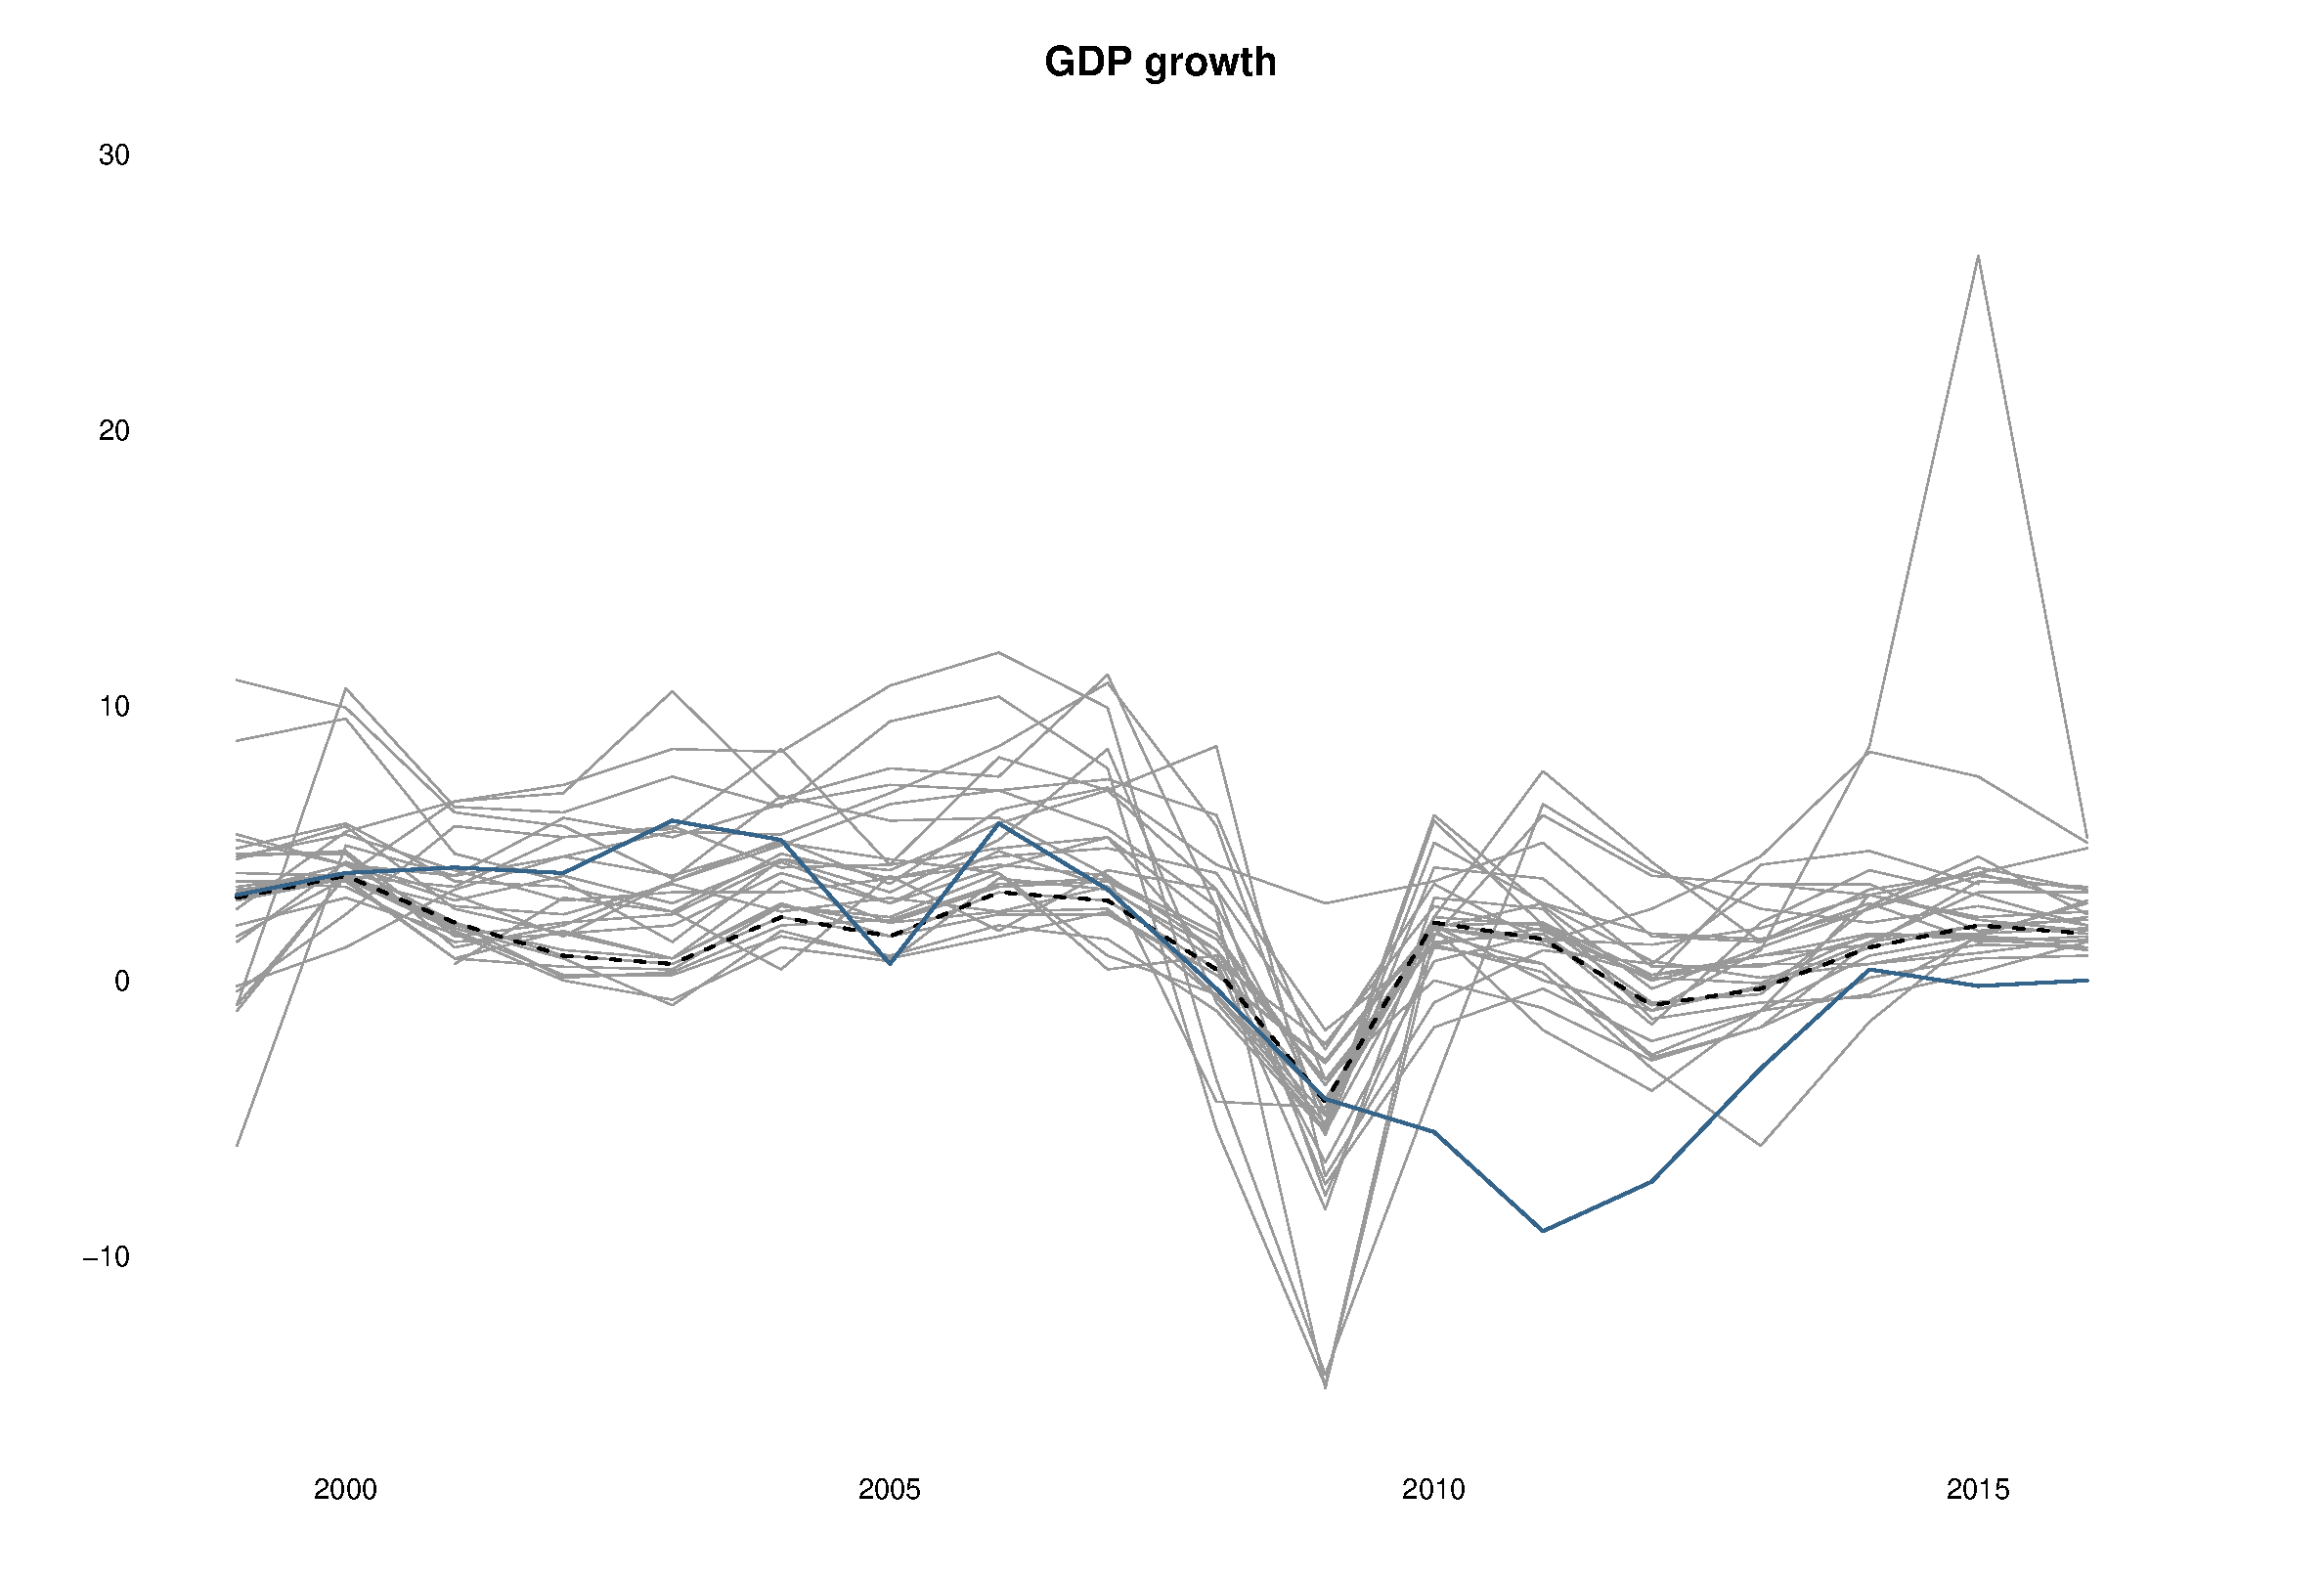
\includegraphics[scale=.3]{gdp_growth.eps}
  \end{figure}
\end{frame}
%--------------------------------------

%--------------------------------------
\begin{frame}
  \begin{figure}
    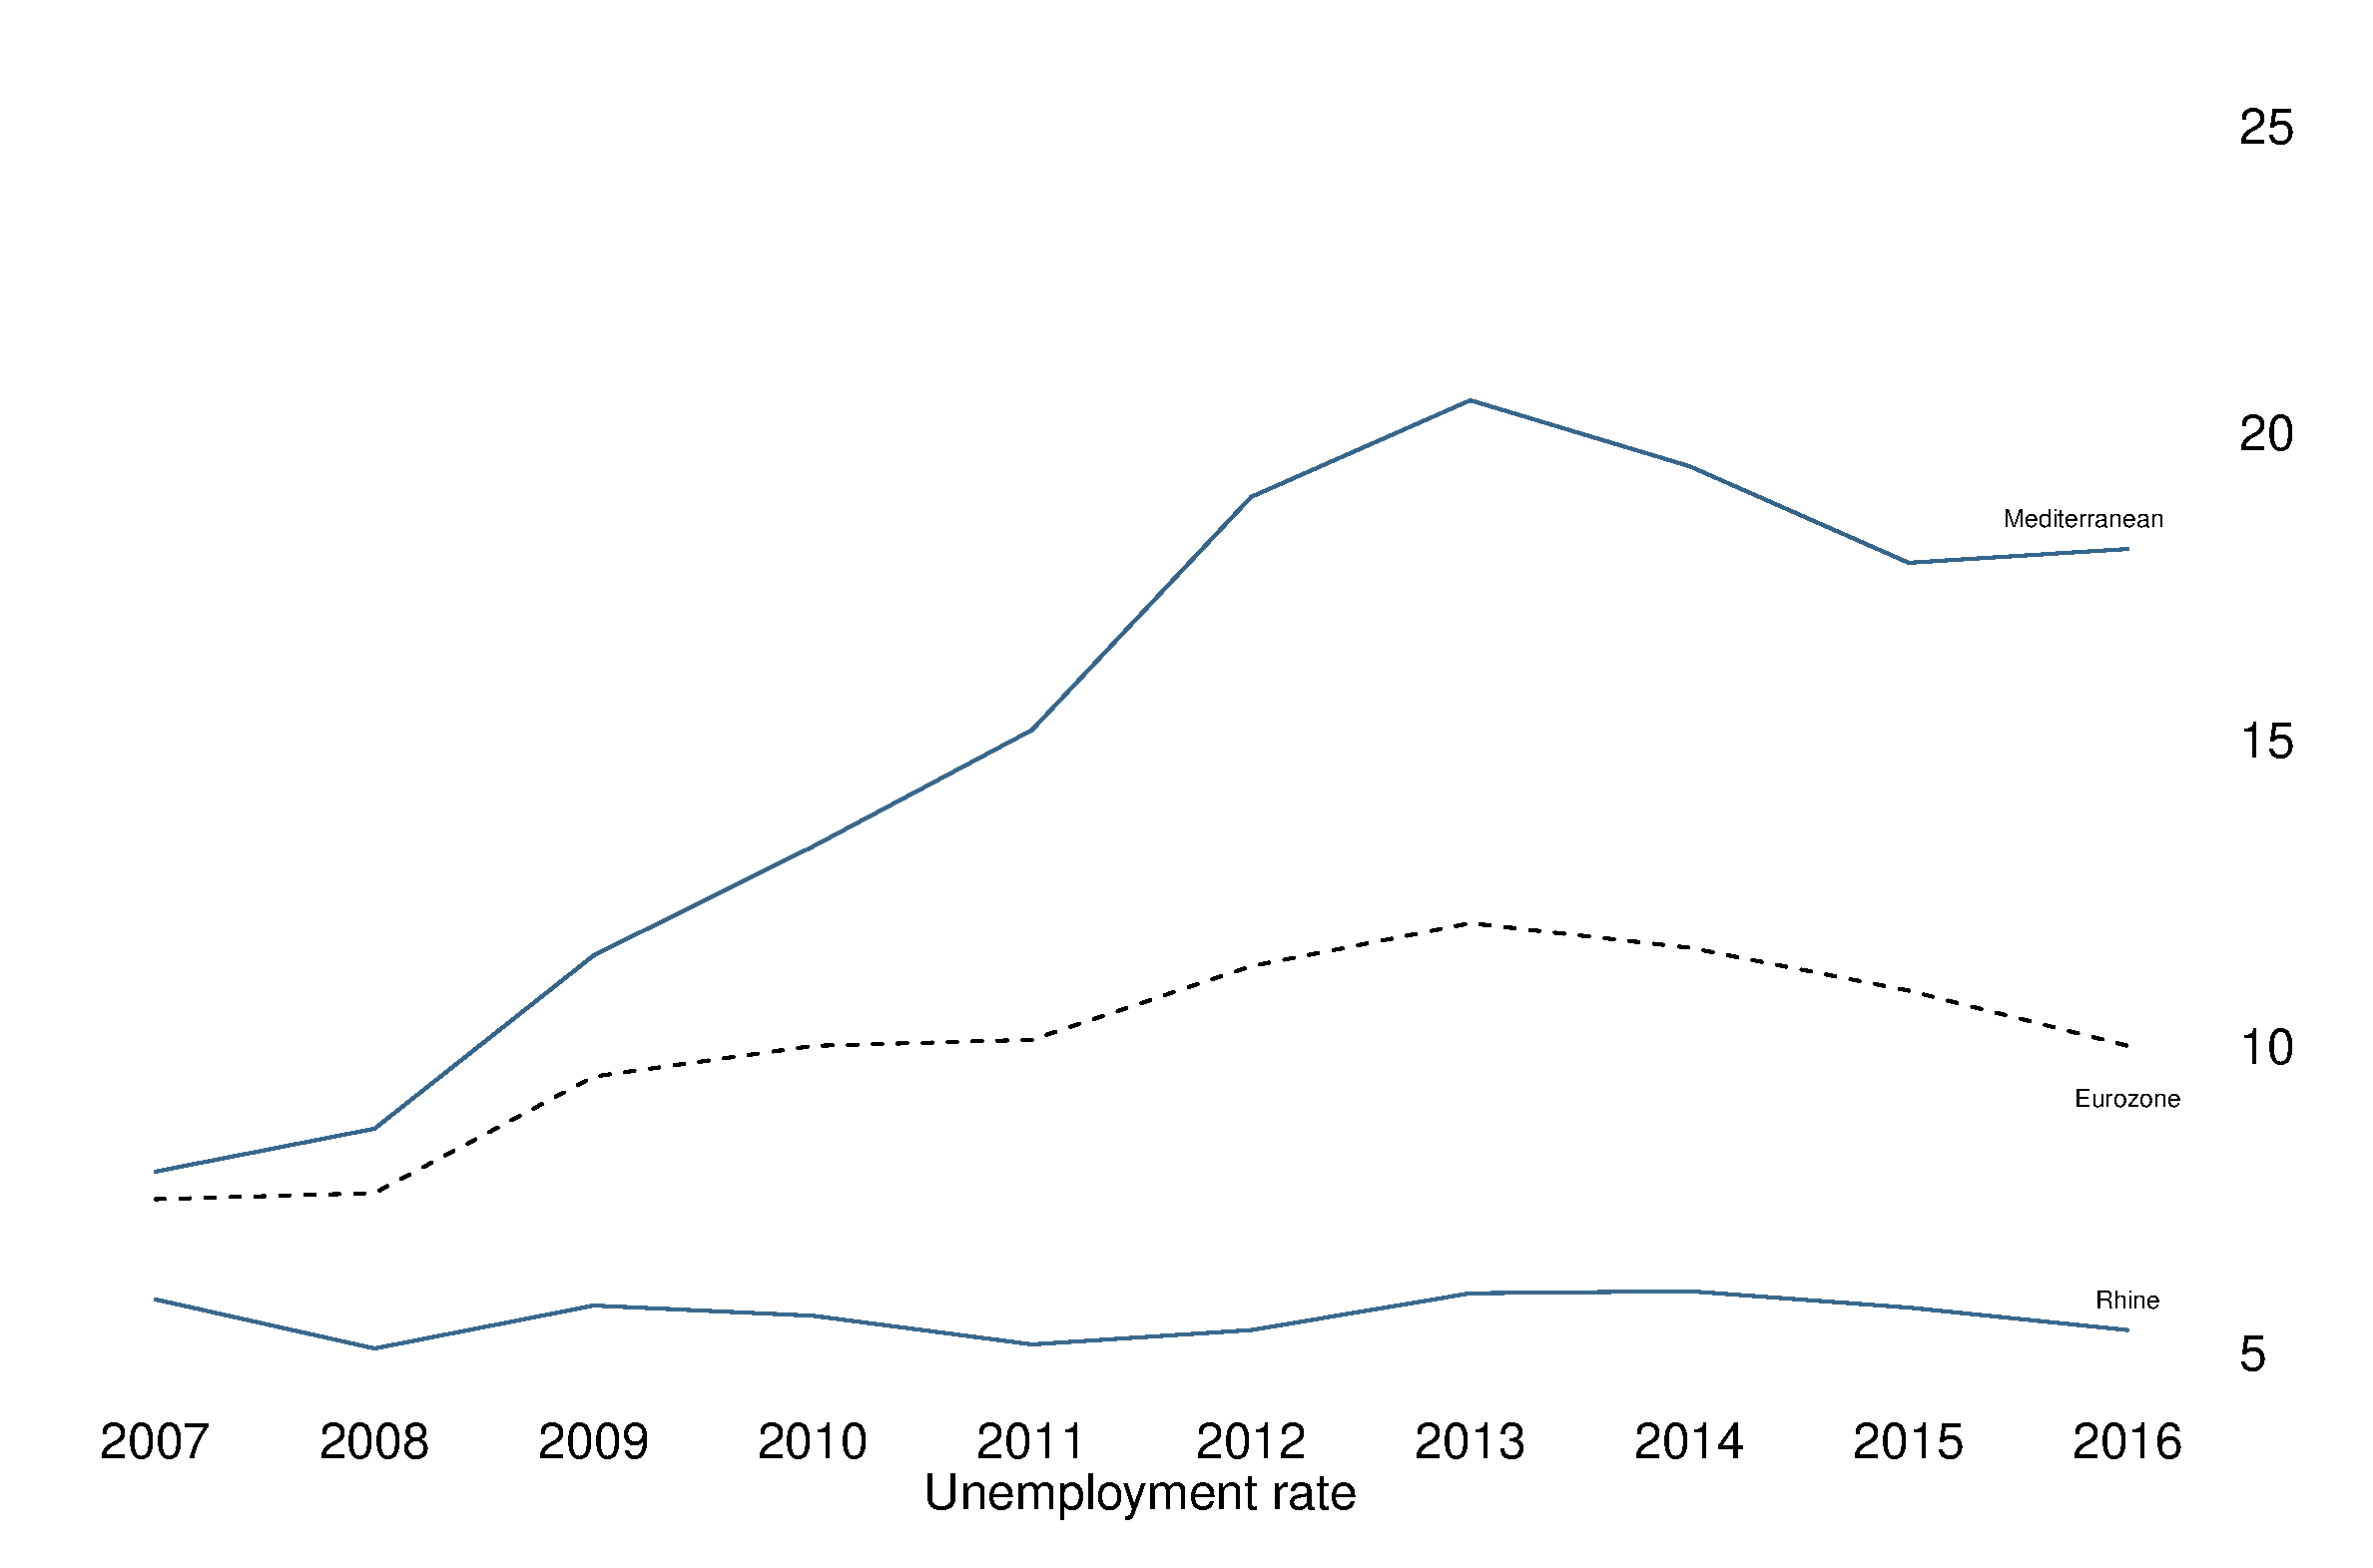
\includegraphics{unemployment.eps}
  \end{figure}
\end{frame}
%--------------------------------------

  
%--------------------------------------
\begin{frame}
  \begin{figure}
    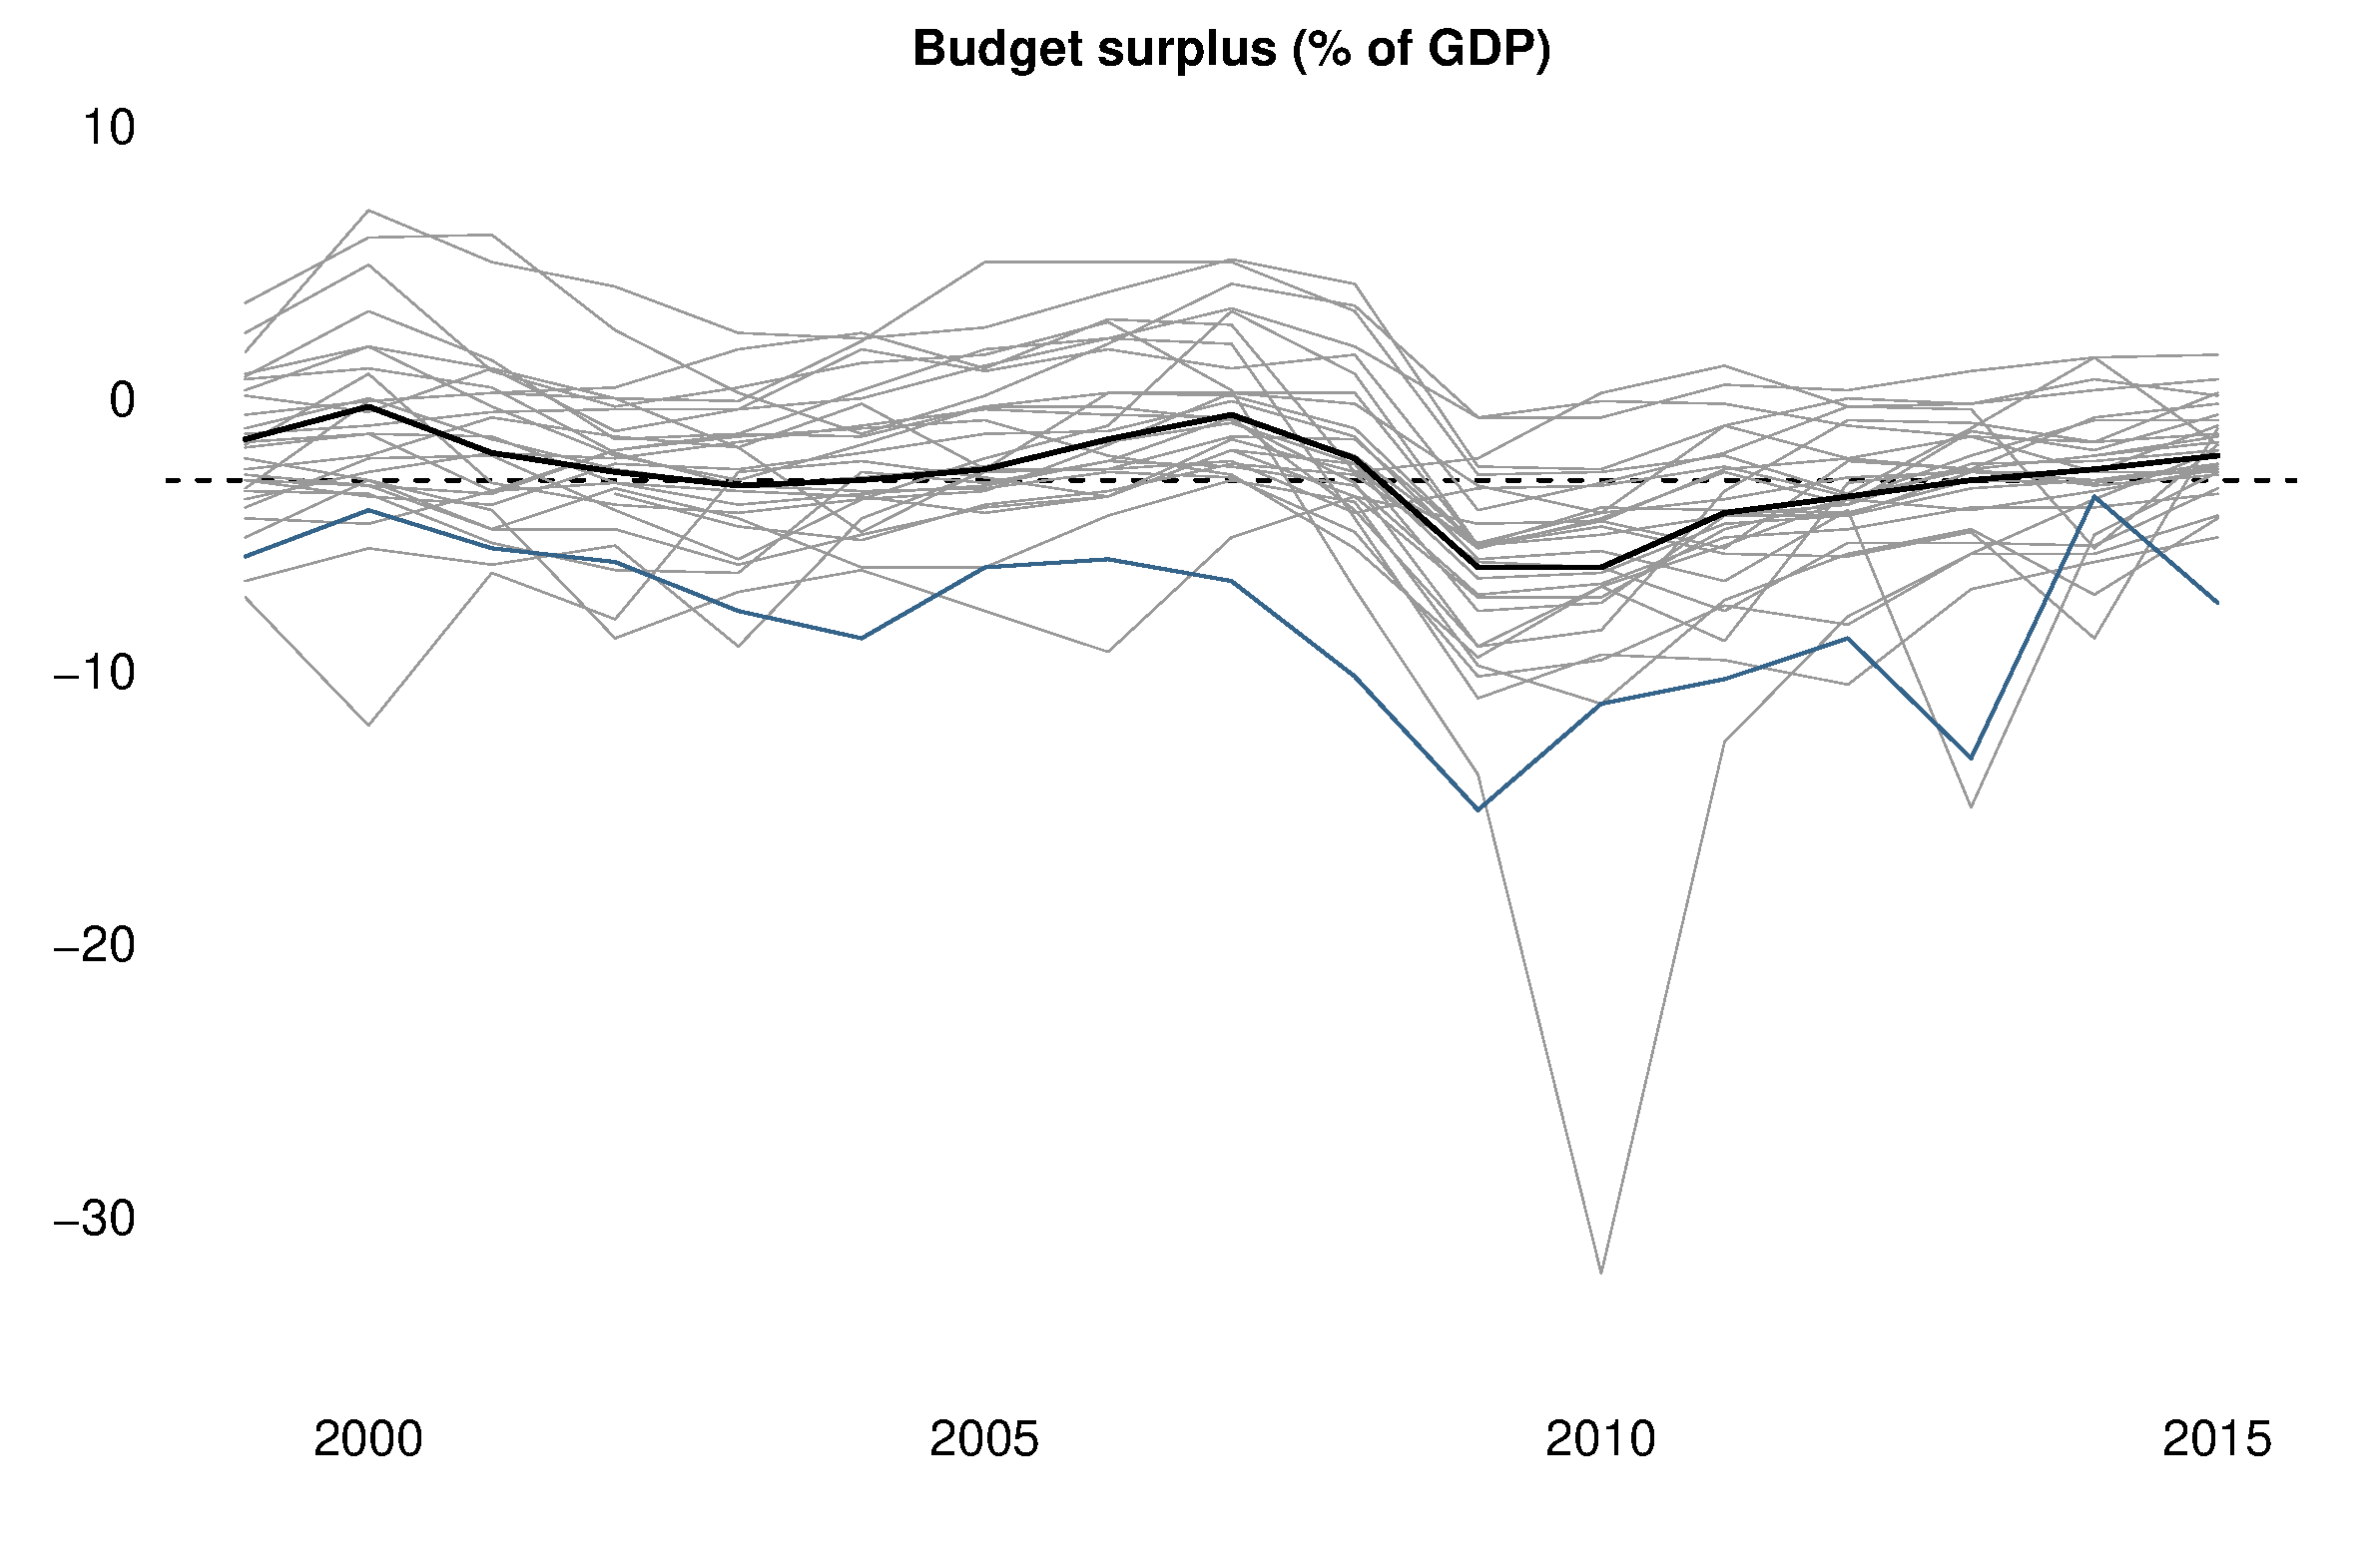
\includegraphics{budget_surplus.eps}
  \end{figure}
\end{frame}
%--------------------------------------

%--------------------------------------
\begin{frame}
  \begin{figure}
    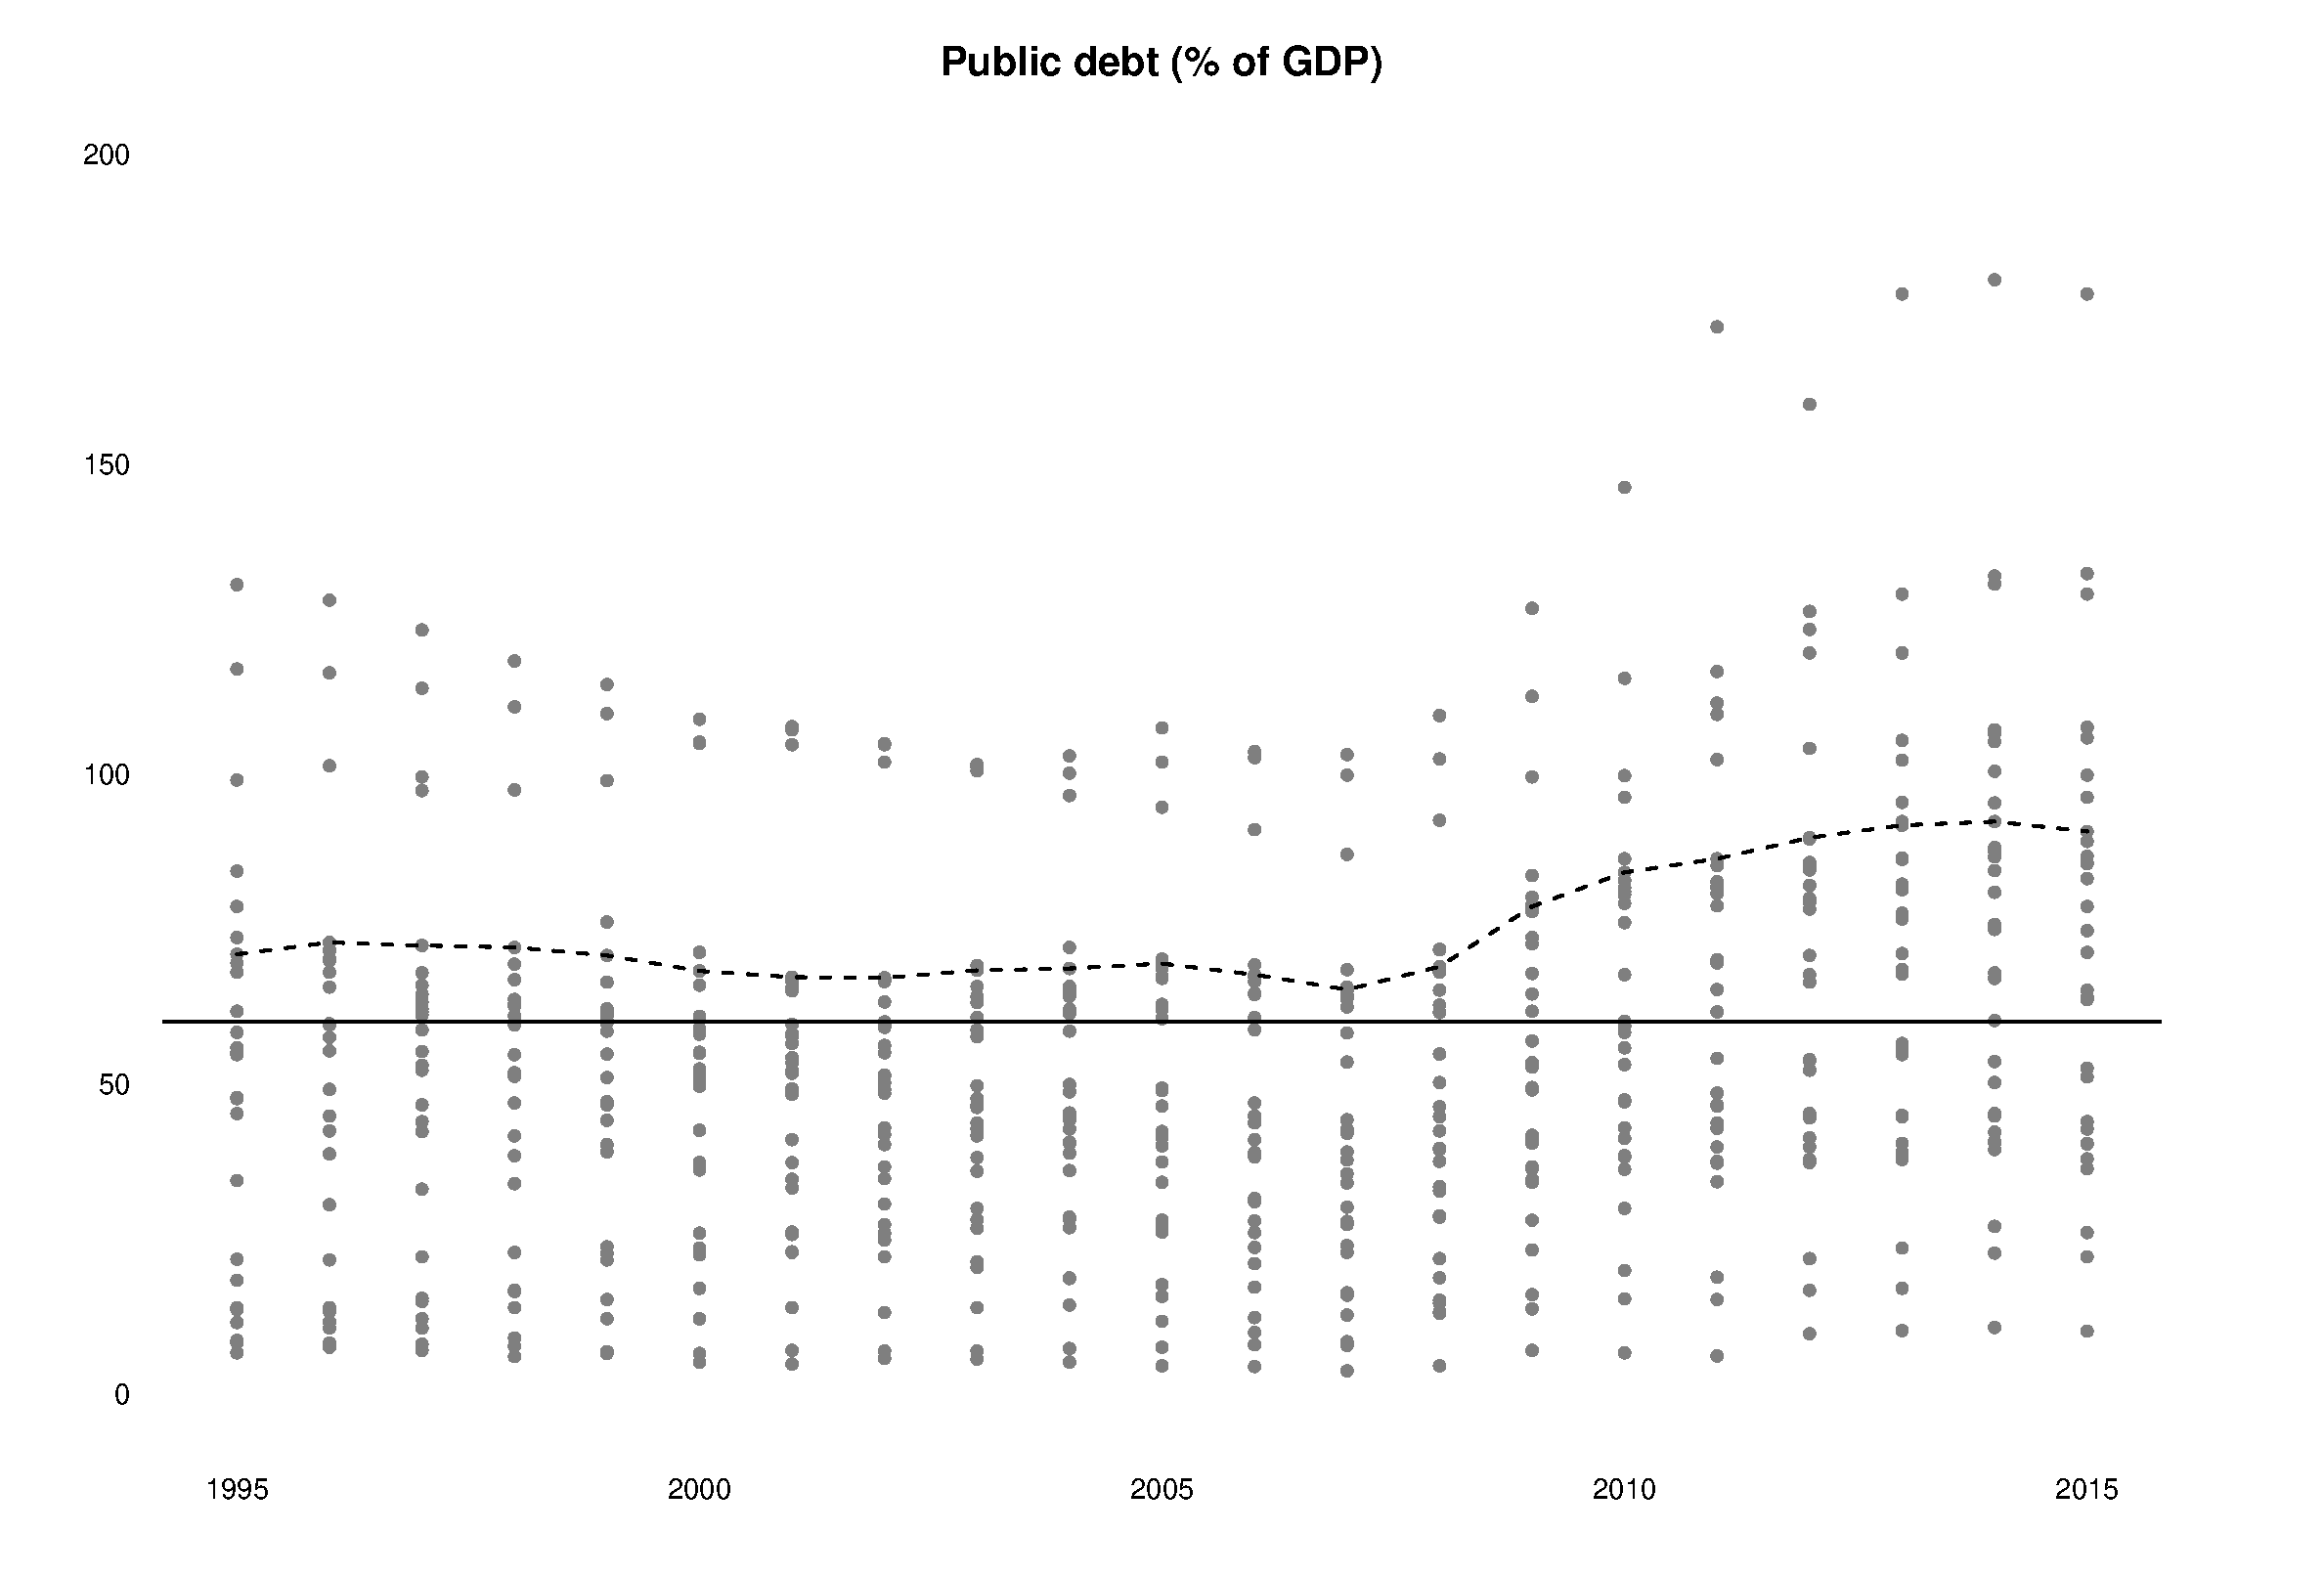
\includegraphics{public_debt2.eps}
  \end{figure}
\end{frame}
%--------------------------------------

%--------------------------------------
\begin{frame}
  Eurocrisis made two things very clear
  \begin{enumerate}
    \item Euro design faults
    \item Political inertia
  \end{enumerate}
\end{frame}
%--------------------------------------

%--------------------------------------
\begin{frame}
  \textbf{Euro design faults}\\
  Euro is currency union with common monetary but not fiscal policy
  \begin{itemize}
    \item Complicates matters in terms of crisis response
    \item Even with EU coordination on fiscal policy (discrepancies in debt levels)
  \end{itemize}
  \medskip
  Since ECB sets monetary policy, countries cannot devalue their currency to regain competitiveness 
\end{frame}
%--------------------------------------

%--------------------------------------
\begin{frame}

\end{frame}
%--------------------------------------

%--------------------------------------
\begin{frame}
  \textbf{Inflation differences}\\
  Optimum currency area theory emphasised risk of asymmetric shocks
  \begin{itemize}
    \item Certainly the effects of the Great Recession has had very divergent effects across the Eurozone
  \end{itemize}
  \medskip
  One issue here is the inflation rate 
  \begin{itemize}
    \item Countries such as Greece and Italy have had persistently higher inflation rates compared to for instance Germany
  \end{itemize}
  \medskip
  With common currency problem is that a country with high inflation rates will see a loss in competitiveness as the real exchange rate appreciates. 
\end{frame}
%--------------------------------------

%--------------------------------------
\begin{frame}
  Consider one good which is sold in two countries
  \begin{enumerate}
    \item Italy
    \item Germany
  \end{enumerate}
  Price in Italy is
  \begin{align}
    p
  \end{align}
  For Germany
  \begin{align}
    p^*
  \end{align}
  Prior to euro could compare price using exchange rate $E$; real exchange rate given by
  \begin{align}
    \frac{Ep}{p^*}
  \end{align}
	With euro $E$ is fixed; inflation will cause increase in 
	\begin{align}
	  \frac{p}{p^*}
	\end{align}
	Appreciation in 
	\begin{align}
	  \frac{Ep}{p^*}
	\end{align}
	Meaning loss in competitiveness. 
\end{frame}
%--------------------------------------

%--------------------------------------
\begin{frame}
  Some explanations for the divergence in inflation rates include
\begin{itemize}
  \item Balassa-Samuelson effect, i.e. inflation rates sign of increase in competitiveness 
  \item ECU fixed at wrong rates
  \item Autonomous wage and price setting
  \begin{itemize}
    \item Wage increases caused by factors other than labour productivity decreases competitiveness
    \item e.g. raising minimum wage, bargaining by sectors that don't face much competition such as civil servants, administered prices in transport and energy
  \end{itemize}
  \item Mistakes in policy
  \begin{itemize}
    \item Government could increase prices and wages through for instance expansionary fiscal policies
  \end{itemize}  
  \item Different preferences
  \begin{itemize}
    \item A country poor at collecting taxes might prefer inflation tax or seigniorage
    \item Variation in consumption baskets can cause different inflations across countries with same monetary policy
  \end{itemize}
\end{itemize}
\end{frame}
%--------------------------------------


%--------------------------------------
\begin{frame}
  \textbf{Political inertia}\\
  Number of negotiation rounds which led to kicking the can further down the road
  \begin{itemize}
    \item Bail outs granted but no structural reforms implemented
    \item Recall no fiscal transfers?
  \end{itemize}
  \medskip
  Symmetric shock led to asymmetric effects
  \begin{itemize}
    \item Differences across countries on desired approach to deal with problem
  \end{itemize}
\end{frame}
%--------------------------------------

%--------------------------------------
\begin{frame}
  Number of factors that worsened the Great Recession in Europe
  \begin{enumerate}
    \item Level of public debt
    \item Trade imbalances
    \item Financial integration
  \end{enumerate}
\end{frame}
%--------------------------------------

%--------------------------------------
\begin{frame}
  \begin{figure}
    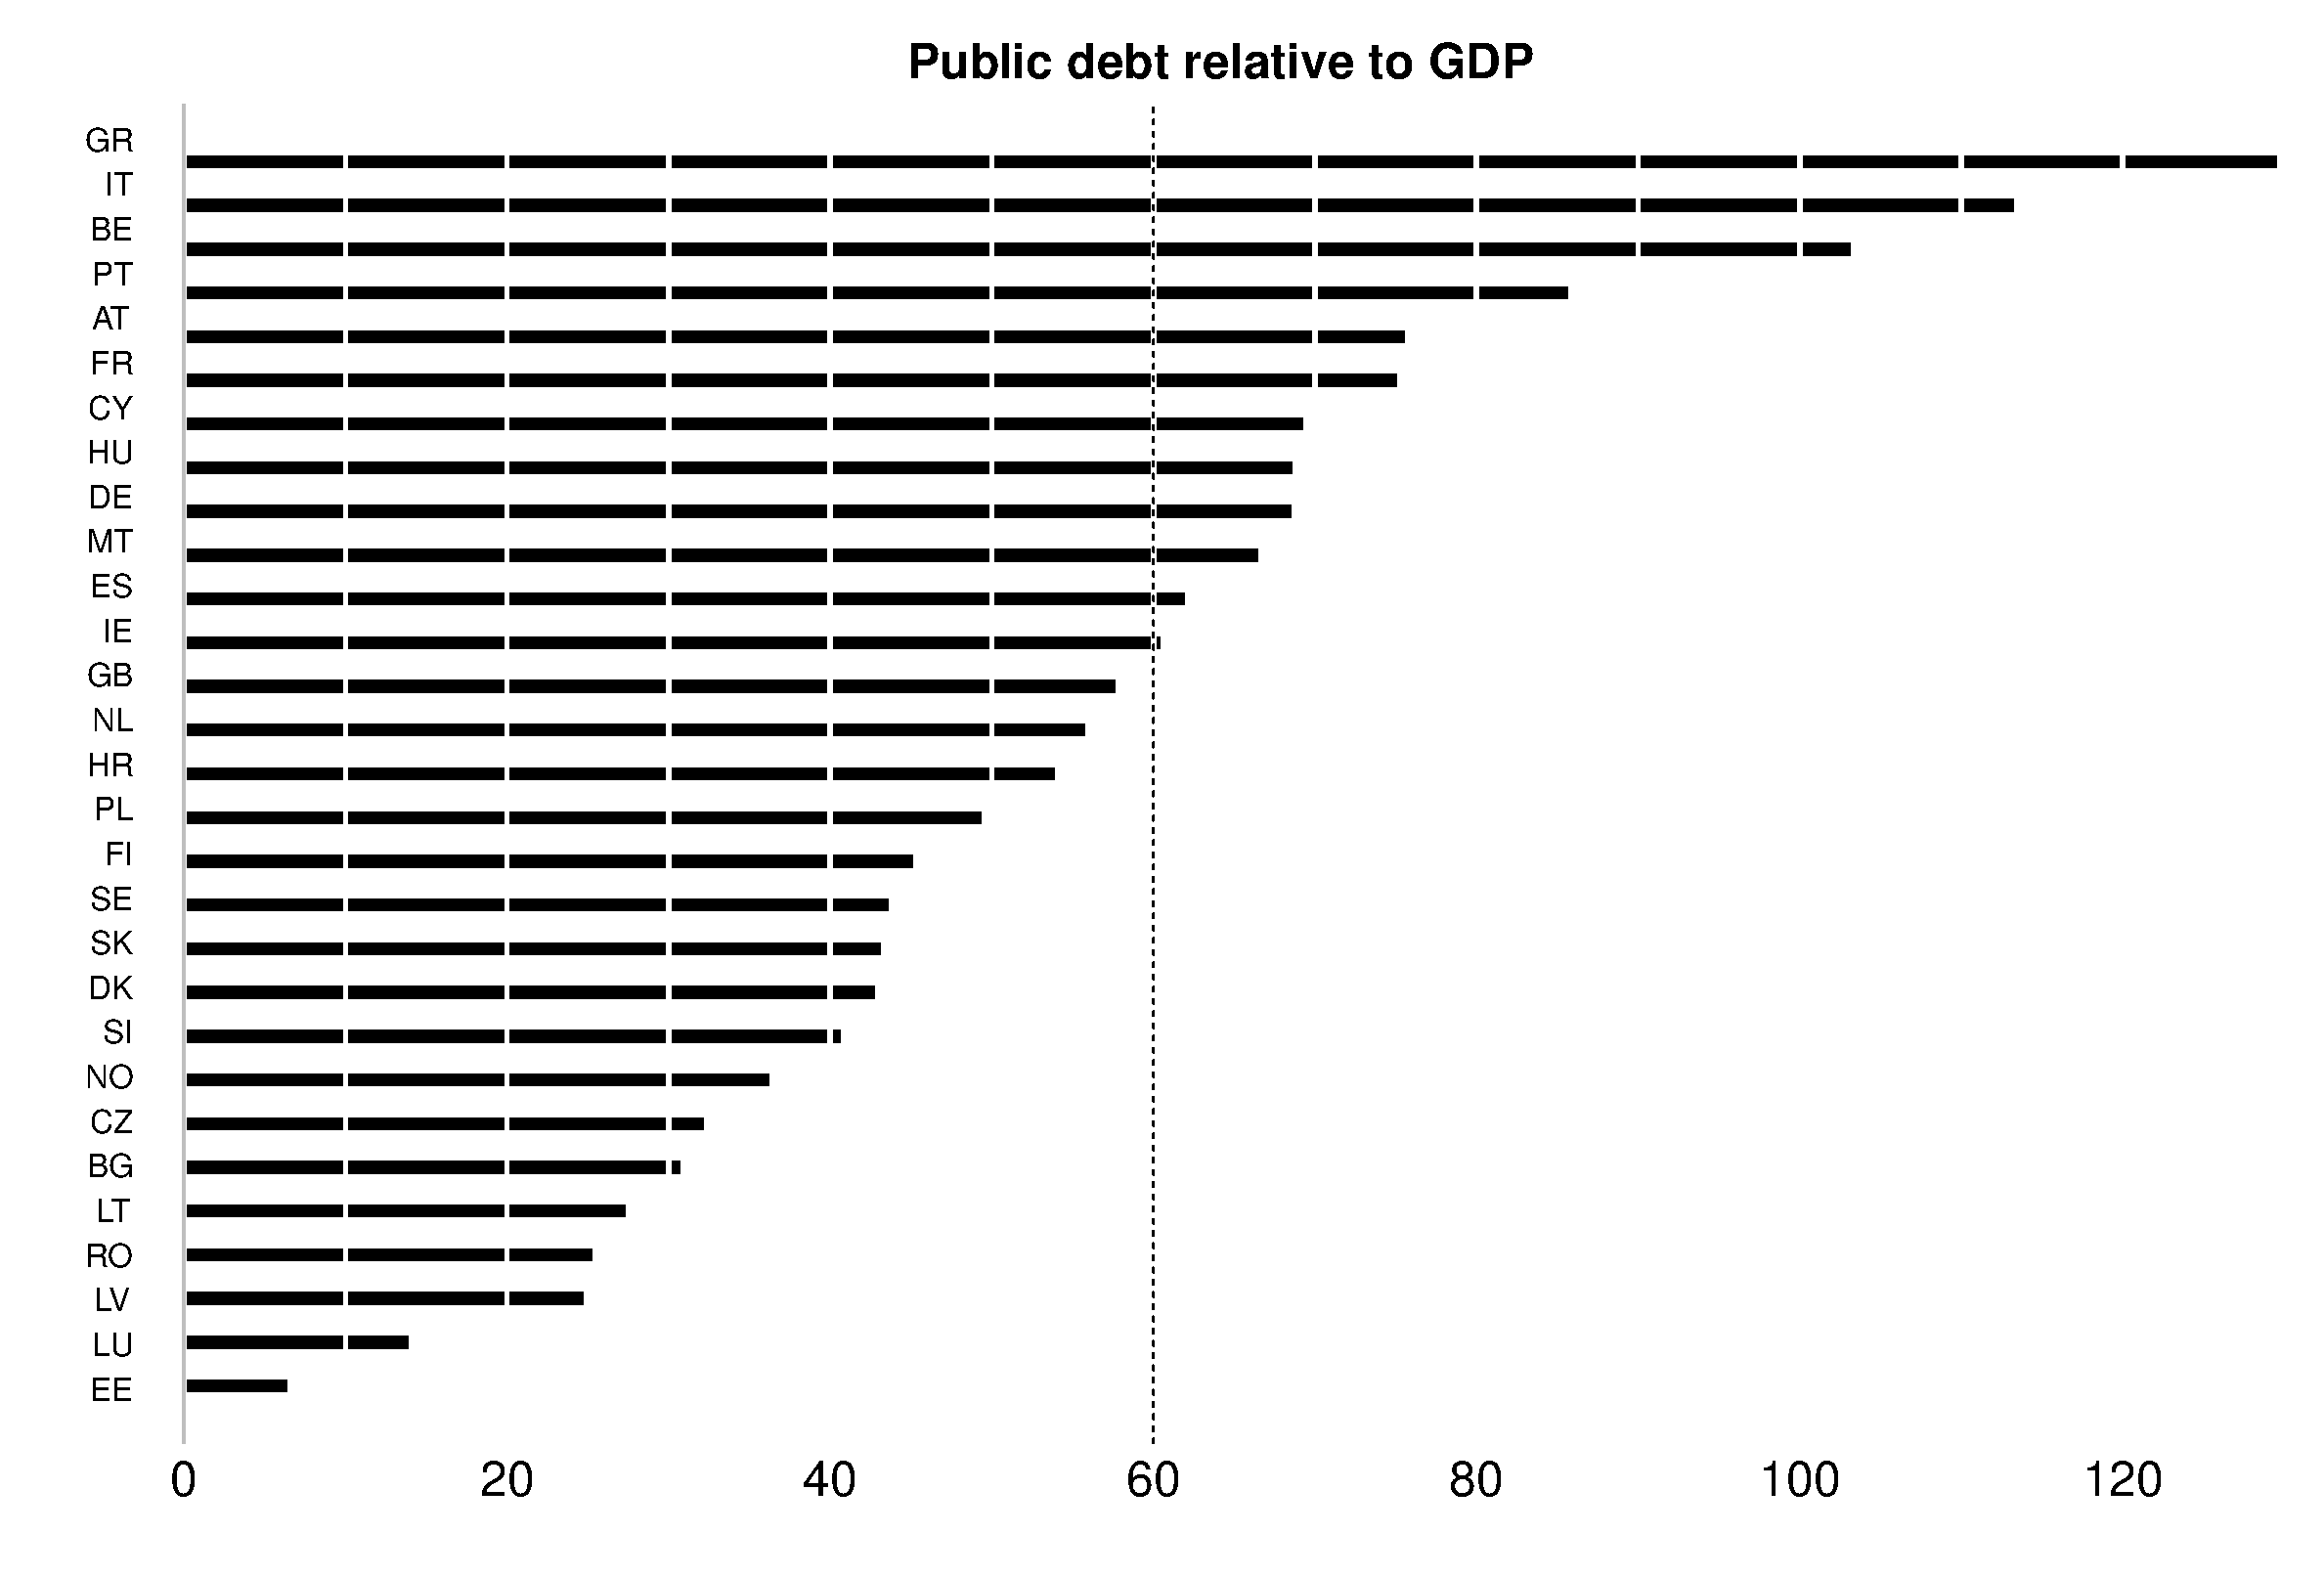
\includegraphics[scale=.3]{public_debt.eps}
  \end{figure}
\end{frame}
%--------------------------------------

%--------------------------------------
\begin{frame}
  \begin{figure}
    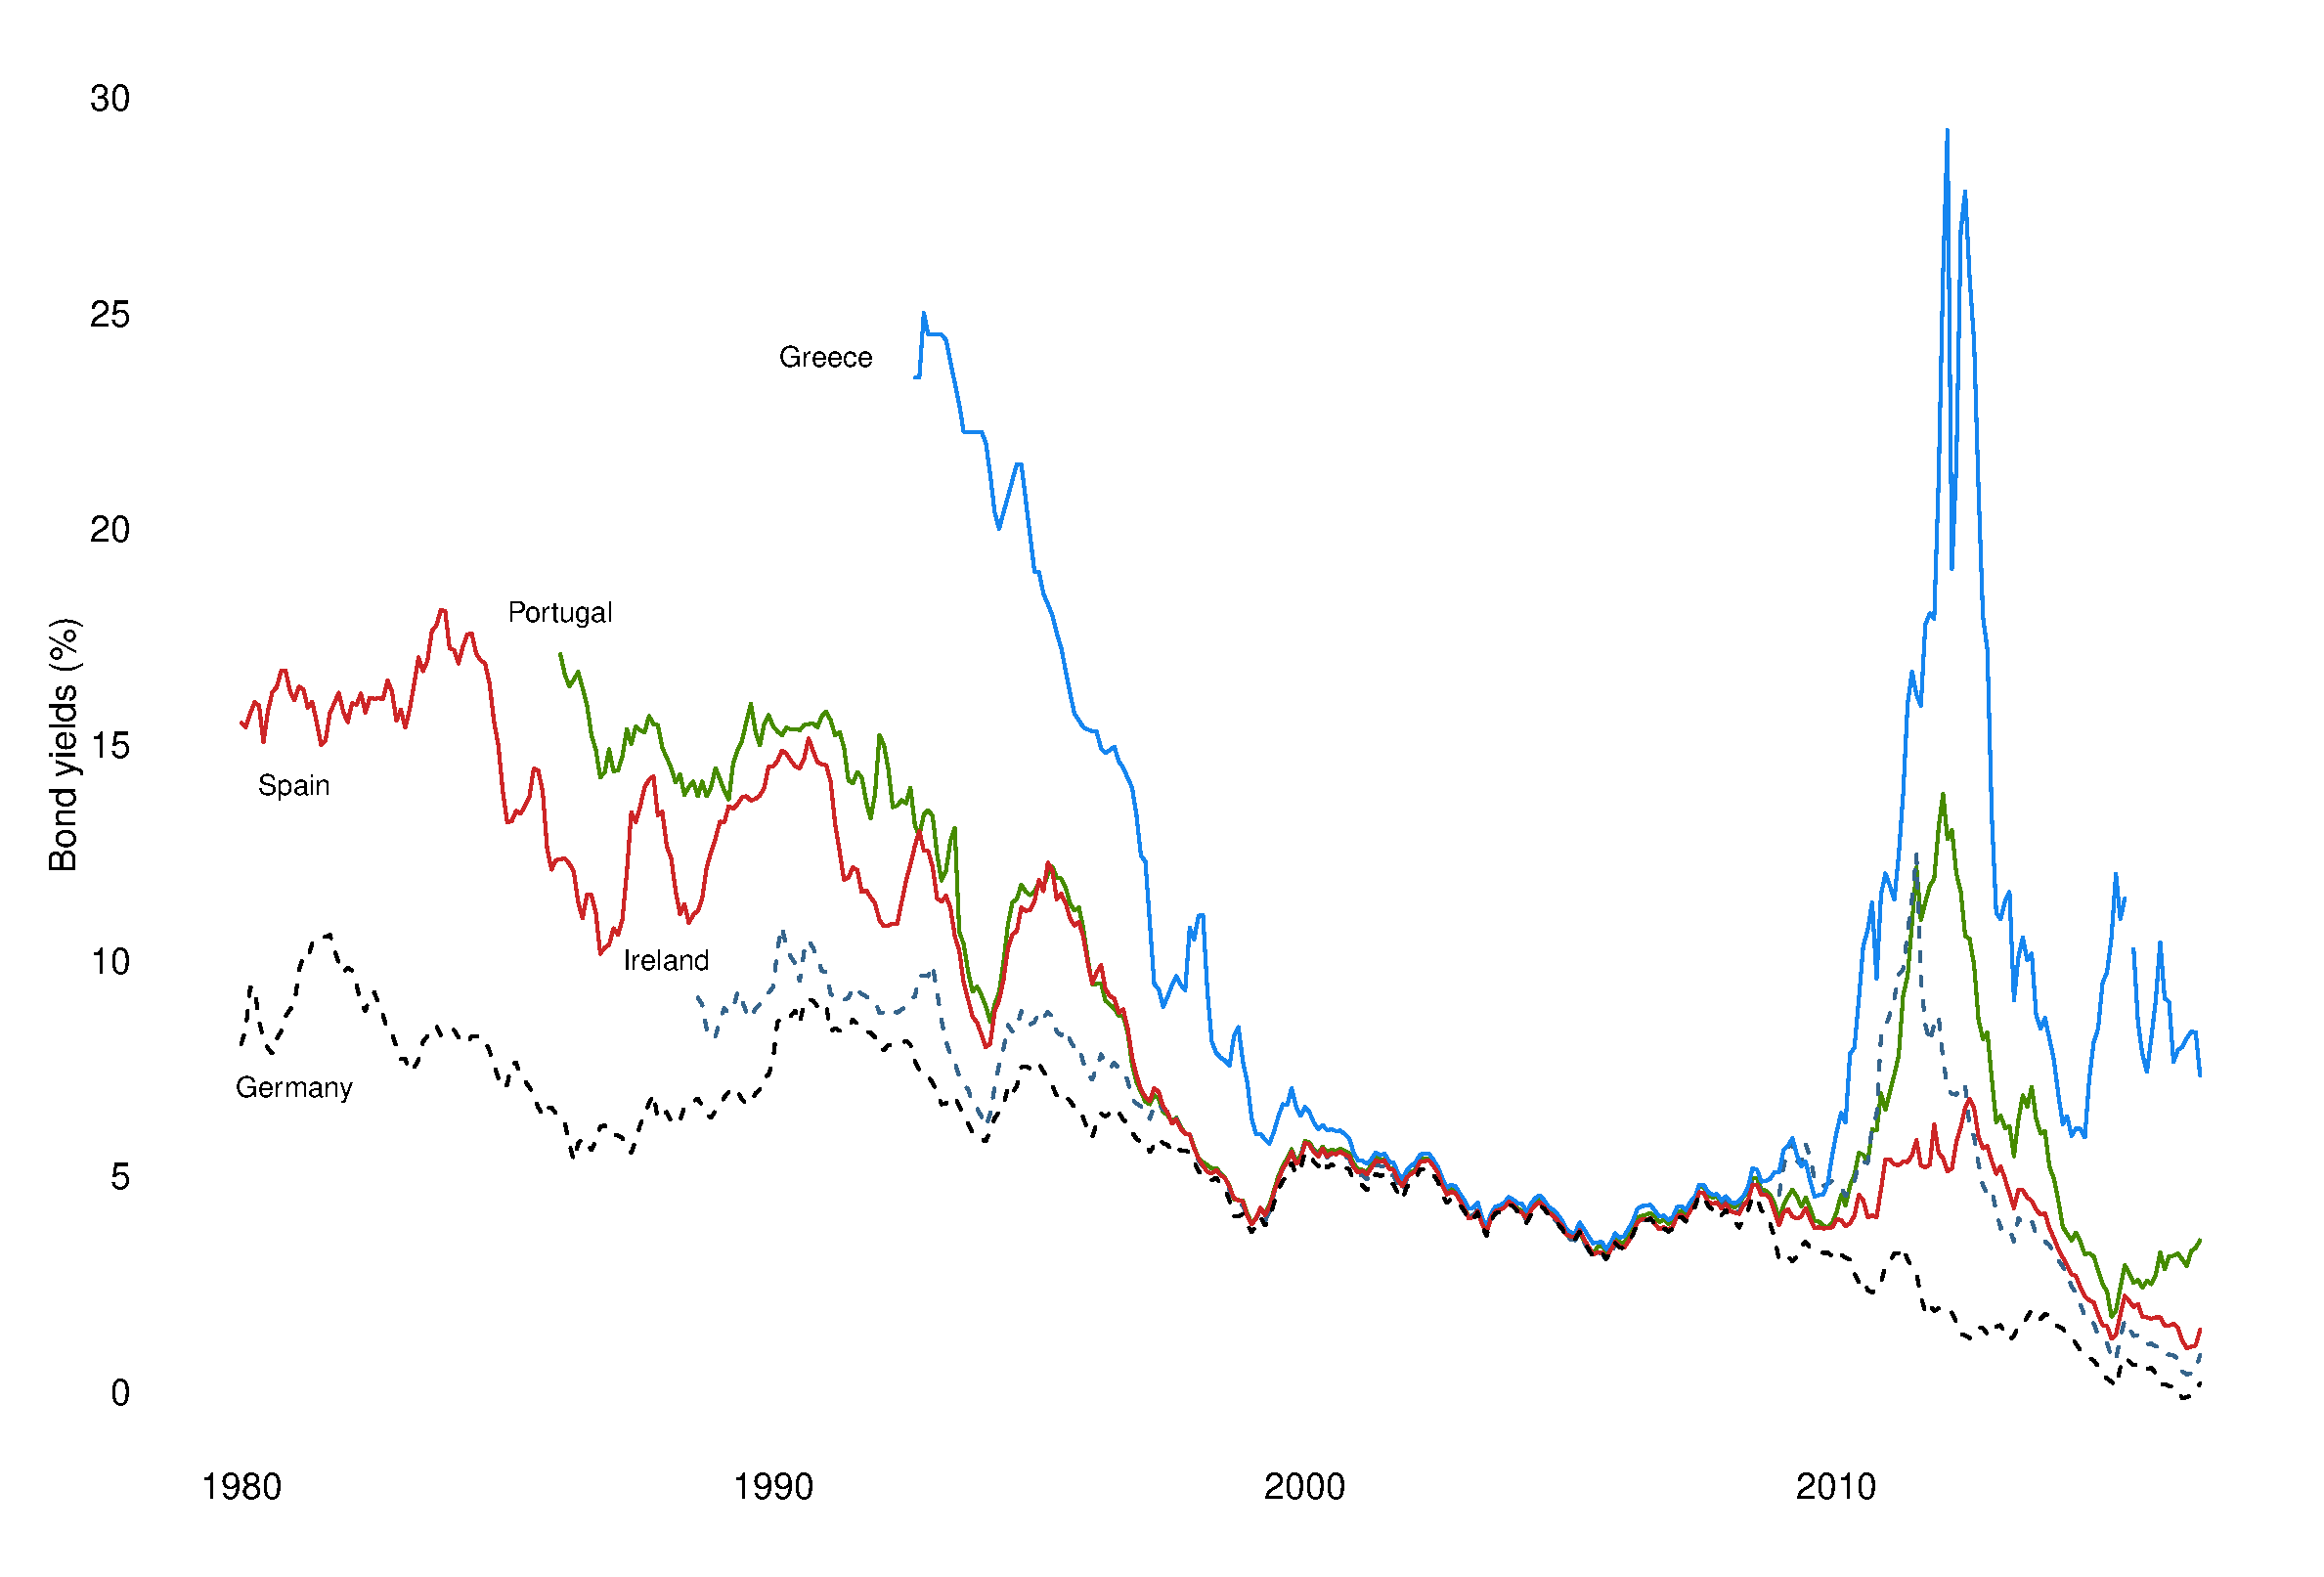
\includegraphics[scale=.3]{bonds.eps}
  \end{figure}
\end{frame}
%--------------------------------------

%--------------------------------------
\begin{frame}
  \begin{figure}
    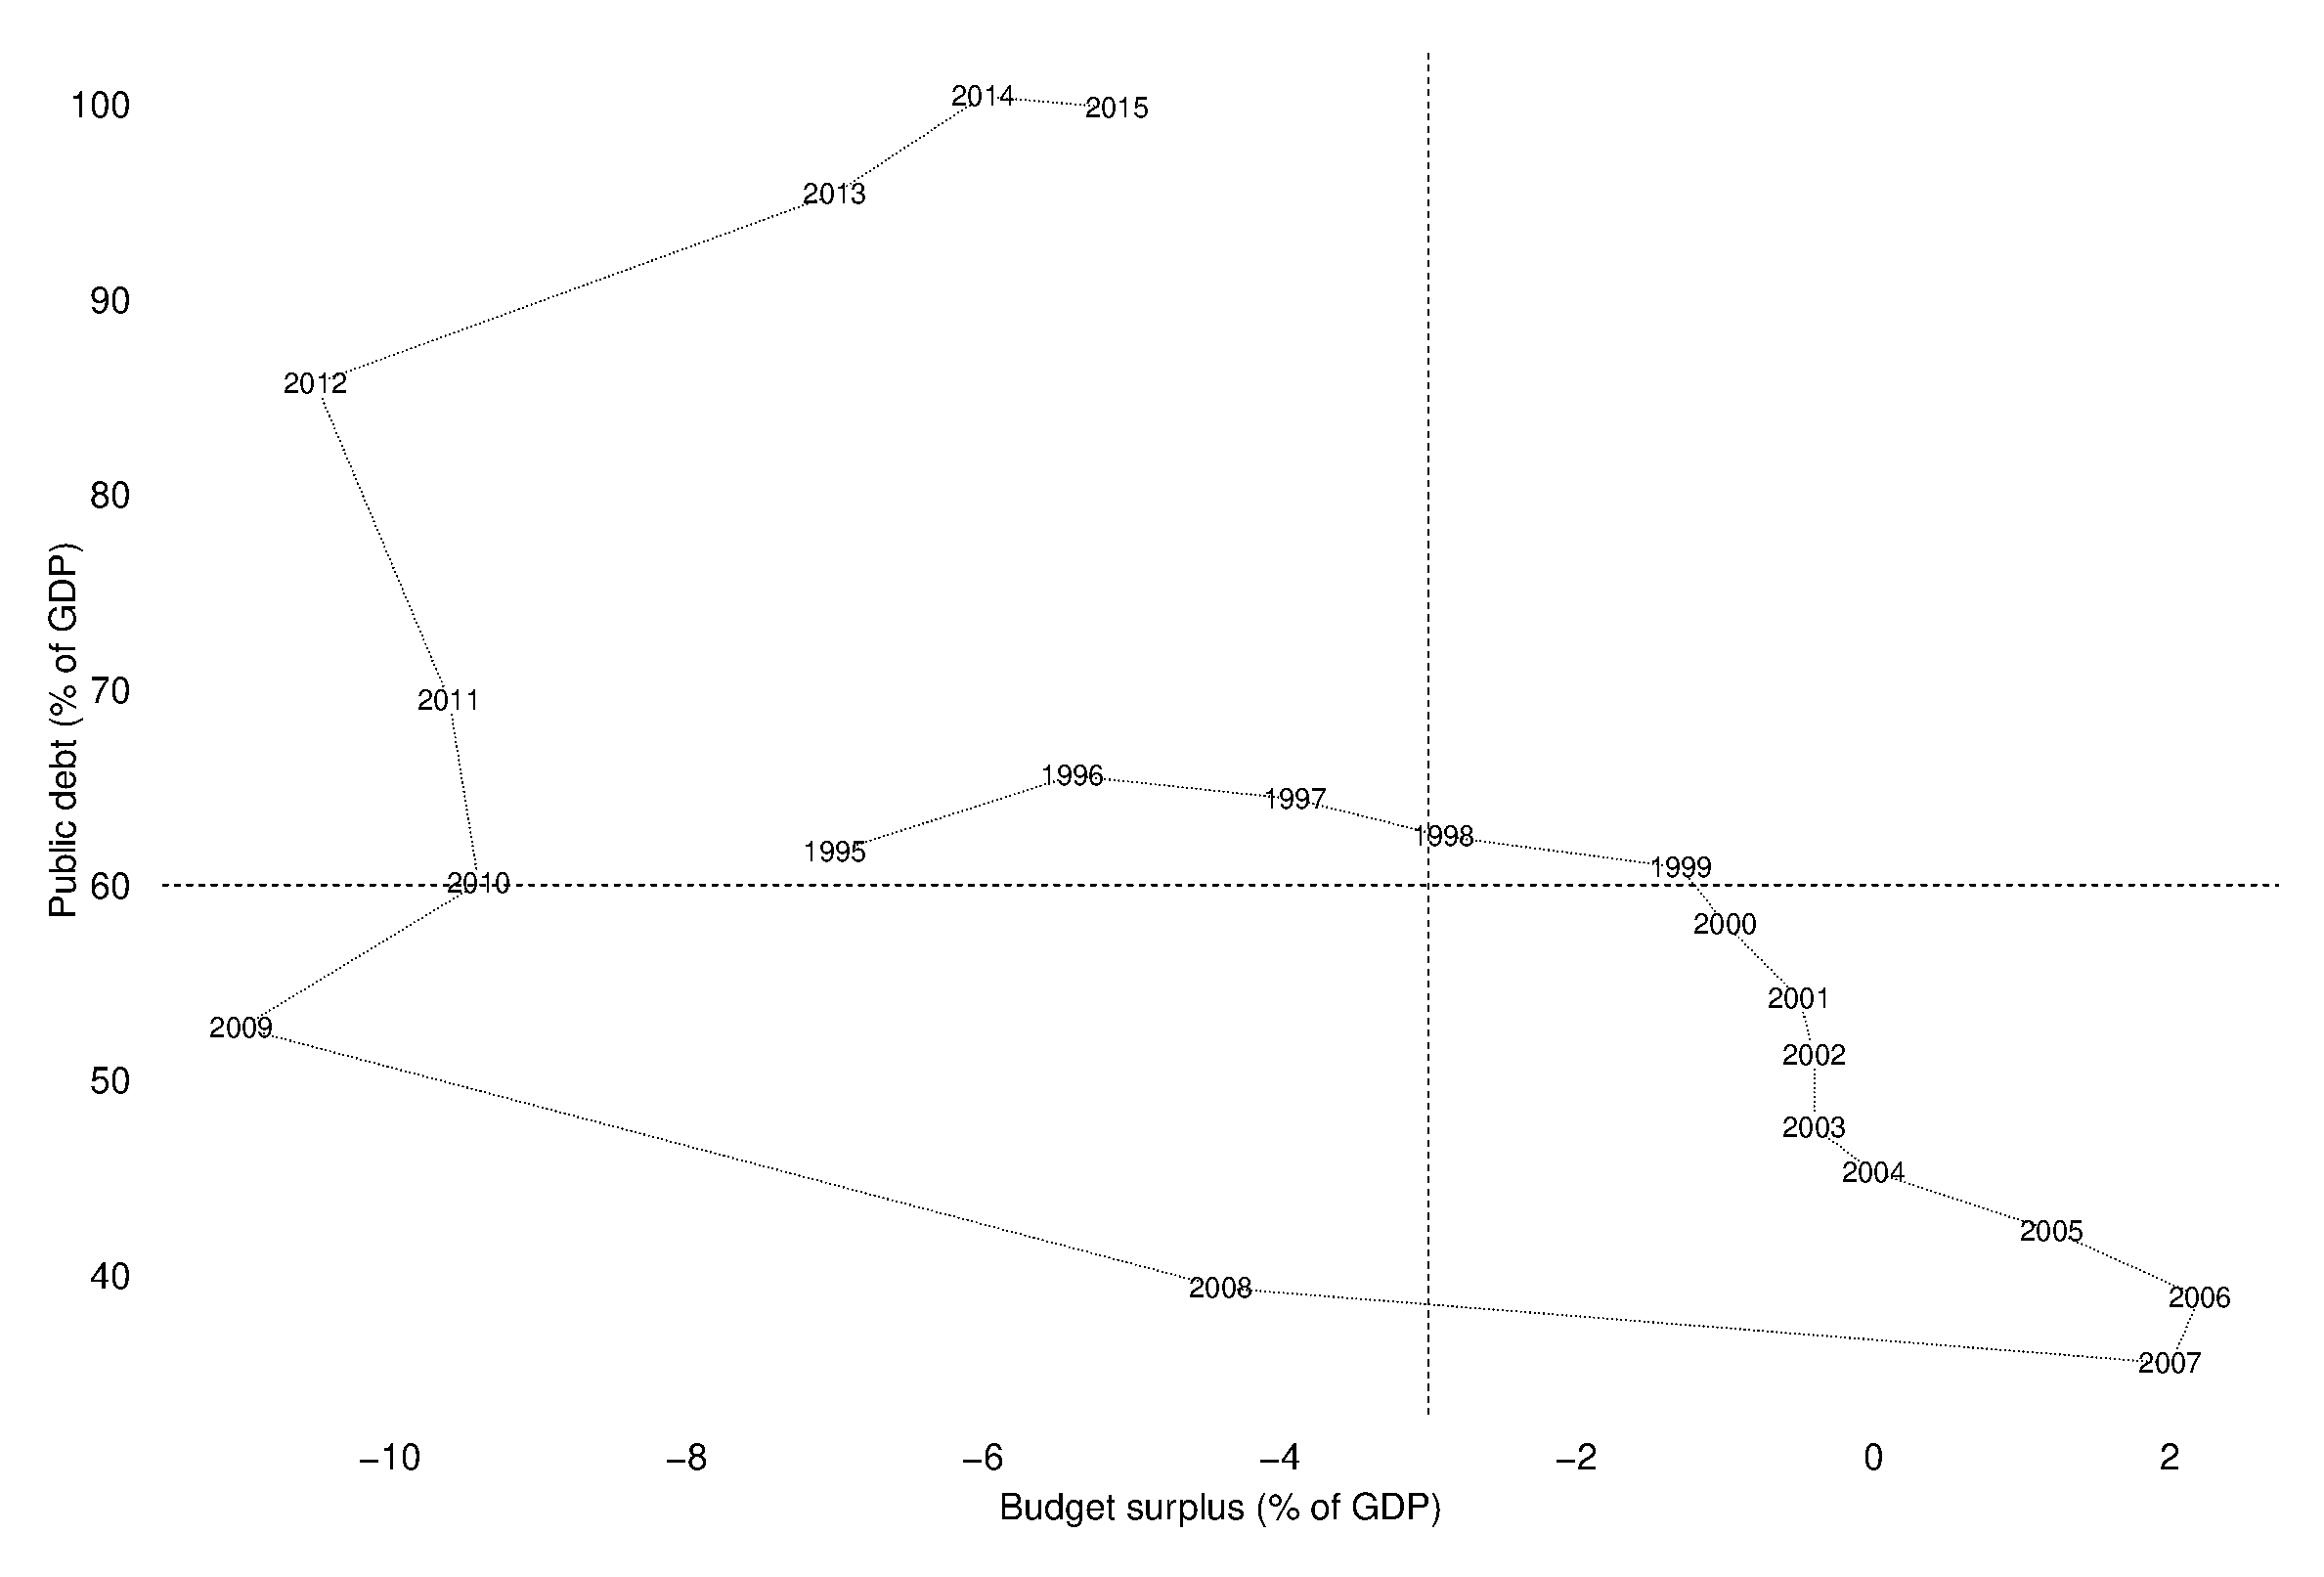
\includegraphics[scale=.3]{spain.eps}
  \end{figure}
\end{frame}
%--------------------------------------

%--------------------------------------
\begin{frame}
  \begin{figure}
    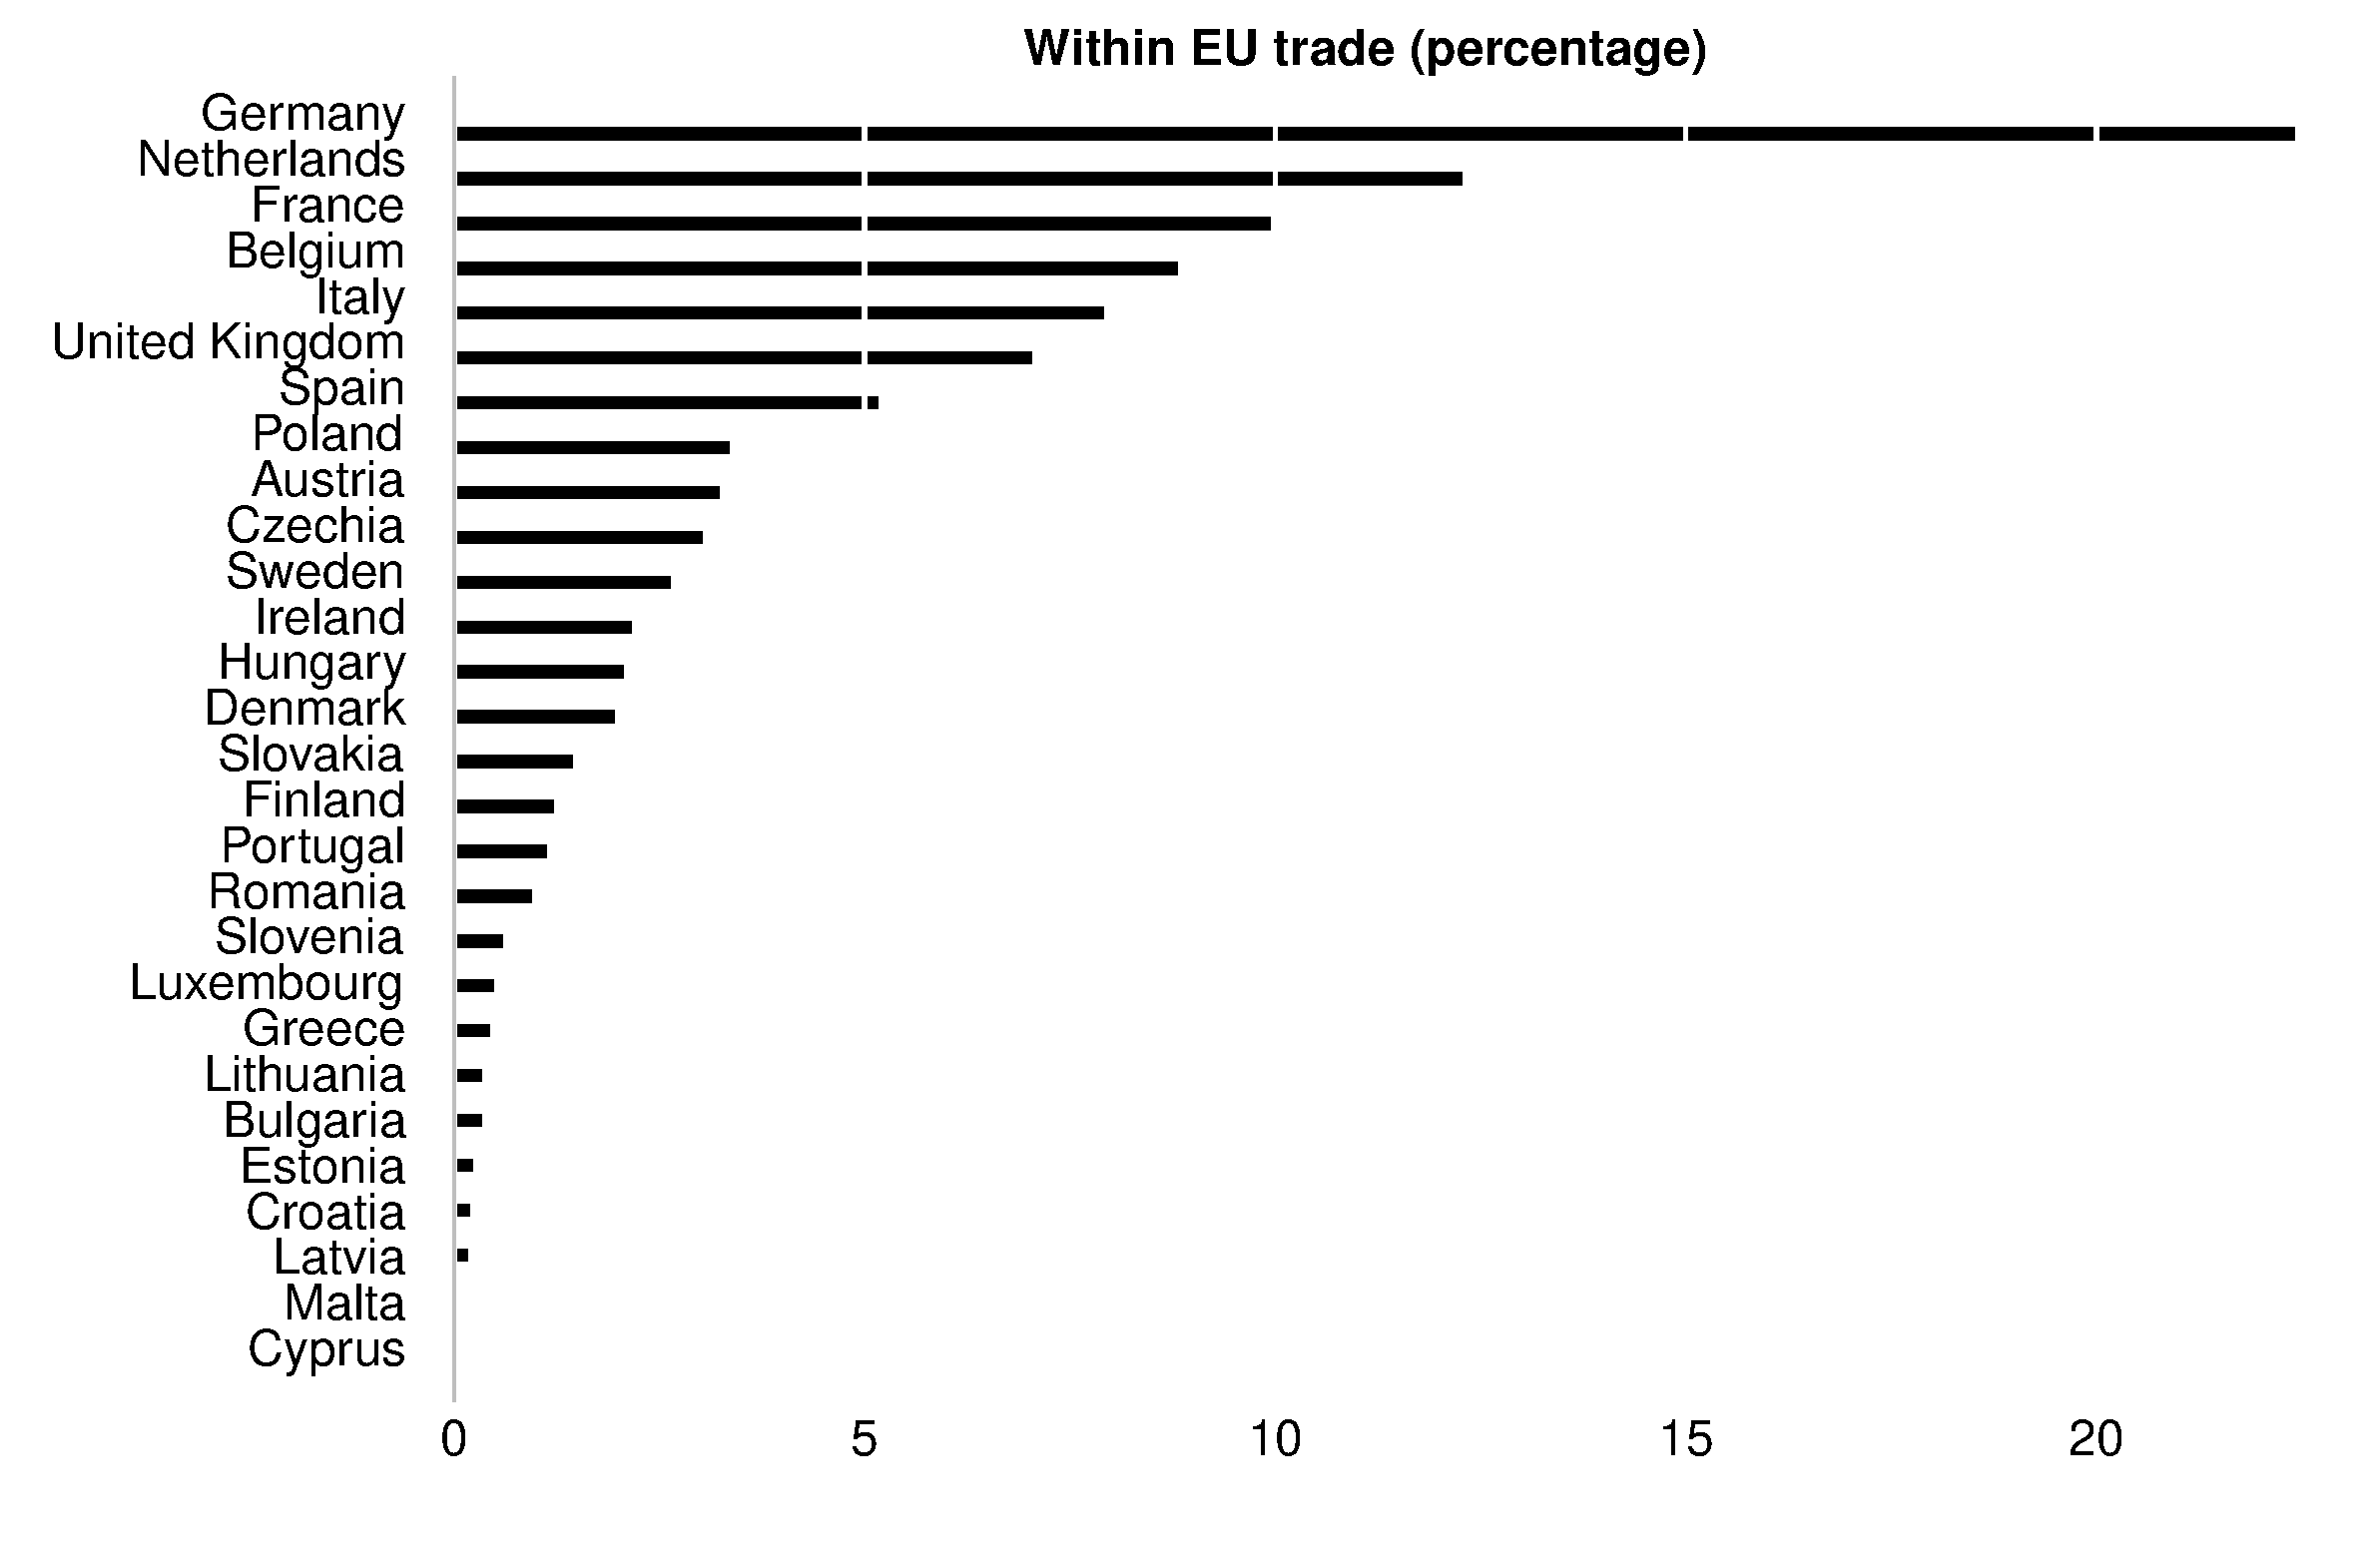
\includegraphics[scale=.3]{within_trade.eps}
  \end{figure}
\end{frame}
%--------------------------------------

%--------------------------------------
\begin{frame}
  \textbf{Trade imbalances}\\
  Cheap credit allowed countries to buy on loans
  \begin{itemize}
    \item Germany increase in trade surplus
    \item Italy, Spain, etc. increase in trade deficit
  \end{itemize}
  \medskip
  Eurocrisis in this sense is that the peripheral areas of the Eurozone have racked up large debts buying German goods, while now they don't have the money to pay for these goods
  \begin{itemize}
    \item Germany could export relatively cheaply because euro kept prices artificially low since it didn't appreciate
  \end{itemize}
\end{frame}
%--------------------------------------

%--------------------------------------
\begin{frame}
  \begin{figure}
    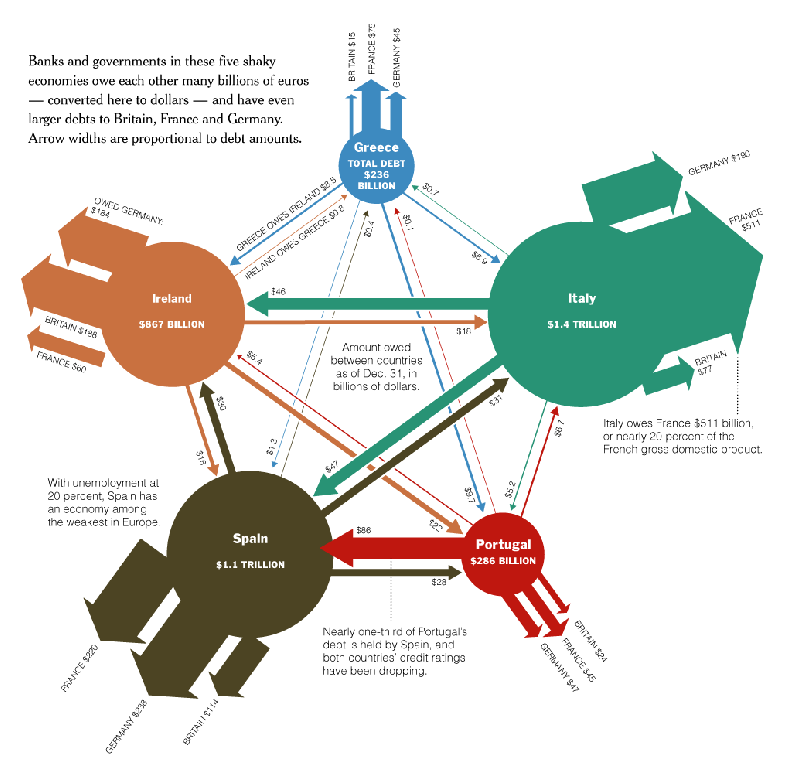
\includegraphics[scale=.2]{debt_nyt.eps}
  \end{figure}
\end{frame}
%--------------------------------------

%--------------------------------------
\begin{frame}
  \textbf{Debt \& deficit}\\
  Straightforward that debt is caused by budget deficits, but how does this work in relation to GDP?\\
  \medskip
  Let $B_t$ bed debt at end of year $t$ in nominal terms; $D_t$ is deficit and will equal
  \begin{align}
    B_t-B_{t-1}=D_t
 \end{align}  
  Let GDP be $Y$\\
  debt/GDP $b_t$\\
  deficit/GDP $d_t$, we get
  \begin{align}
    \frac{B_t-B_{t-1}}{Y_t} &= \frac{D_t}{Y_t}\\ \nonumber
    b_t-\frac{B_{t-1}}{Y_t} &= d_t  
  \end{align}
\end{frame}
%--------------------------------------

%--------------------------------------
\begin{frame}
 Given 
 \begin{align}
   g_t=\frac{Y_t-Y_{t-1}}{Y_t}=\frac{Y_t}{Y_{t-1}}-1
 \end{align}
 Can rewrite
 \begin{align}
   b_t-\frac{B_{t-1}}{Y_t} &= d_t  
 \end{align}
 as 
 \begin{align}
  \frac{B_{t-1}}{Y_t} = \frac{B_{t-1}}{Y_{t-1}}\frac{Y_{t-1}}{Y_t} = \frac{b_{t-1}}{1+g_t} 
 \end{align}
\end{frame}
%--------------------------------------

%--------------------------------------
\begin{frame}
  \begin{align}
    b_t-\frac{b_{t-1}}{1+g_t} &= d_t\\
  b_t-b_{t-1} &= (1+g_t)d_t-g_tb_t  
  \end{align}
  \medskip
  For a constant debt-to-GDP ratio we need $b_t$ to equal $b_{t-1}$ which implies that the deficit-to-GDP ratio equals
\begin{align}
  (1+g_t)d_t-g_tb_t &=0 \\
  dt &= \frac{g_tb_t}{1+g_t} = \frac{g_t}{1+g_t}b_t
\end{align}
\end{frame}
%--------------------------------------


%--------------------------------------
\begin{frame}
  Maastricht Treaty has set convergence criteria to
  \begin{align}
    b_t=60\%\\
    d_t=3\%
  \end{align}
   (X) would be satisfied when growth rate is about 5.3\%
   \begin{itemize}
     \item implicit assumption is that real GDP growth is 3\% and inflation is 2\%, equaling a nominal growth rate of 5\%.  
   \end{itemize} 
   If a country is able to keep the debt level constant then naturally the debt-to-GDP ratio will decrease due to GDP growth. 
   \begin{itemize}
     \item This also implies that the deficit becomes larger at high nominal growth rates.  
   \end{itemize}
\end{frame}
%--------------------------------------


%--------------------------------------
\begin{frame}
  \textbf{EU response}\\
  Economic problem required solution with political backing
  \begin{itemize}
    \item Not easy given break down in confidence between member states
    \item Specifically North vs. South
  \end{itemize}
  \medskip
  Some solutions that didn't make it
  \begin{enumerate}
    \item Eurobonds
    \item Fiscal transfers
    \item Kick Greece out of eurozone
    \item Quantitative easing
  \end{enumerate}
 \end{frame}
%--------------------------------------

%--------------------------------------
\begin{frame}
  \textbf{Eurobonds}
  \begin{itemize}
    \item Allowed governments to refinance debts as high-yield countries benefit from creditworthiness of low-yield countries
    \item Creates a moral hazard problem as it is possible subject to free riding
  \end{itemize}
  \textbf{Fiscal transfers}
  \begin{itemize}
    \item \item Basically rich eurozone countries compensating poor eurozone countries for their losses
    \item No system in place to do this, and would need political backing which is unlikely to be popular with population of richer countries
  \end{itemize}
\end{frame}
%--------------------------------------

%--------------------------------------
\begin{frame}
  \textbf{Greece}
  \begin{itemize}
    \item Return to drachme, Greece would be able to set own monetary policy and regain competitiveness
    \item Would still costs a lot of money to Greece because the debt has to be repaid
    \item Would create undesired precedent and risk stability of the whole euro project
  \end{itemize}
  \textbf{QE}
  \begin{itemize}
    \item Can help boost economic activity
    \item Germany is not a fan of QE 
    \item although the ECB did engage in some form of QE eventually
  \end{itemize}
\end{frame}
%--------------------------------------

%--------------------------------------
\begin{frame}
  EU took following measures (2010)
  \begin{itemize}
    \item European Financial Stability Facility (EFSF) 
    \item European Financial Stabilisation Mechanism (EFSM) 
  \end{itemize}
  These more or less temporary measures were followed up by a more formalised structure to assist eurozone member states under the European Stability Mechanism (ESM) in 2012.
\end{frame}
%--------------------------------------

%--------------------------------------
\begin{frame}
  \textbf{European Financial Stability Facility}\\
  Temporary crisis resolution mechanism for euro area member states financed through the issuance of bonds and other debt instruments
  \begin{itemize}
    \item On international capital markets
    \item Capacity of 500B EU
    \item Guaranteed by other eurozone member states (so sort of eurobonds)
  \end{itemize}
    \medskip
   Assistance was used to provide loans, recapitalise banks, or buy sovereign debt    
   \begin{itemize}
     \item To Ireland, Portugal, Greece
   \end{itemize}
\end{frame}
%--------------------------------------

%--------------------------------------
\begin{frame}
  \textbf{European Financial Stabilisation Mechanism}\\
   Provides financial assistance to any EU member state which is facing severe financial disturbances
   \begin{itemize}
     \item Country can get up to 60B EUR in assistance from the European Commission 
     \item The fund is financed through  bond sales, using EU budget as collateral    
    \item Provided assistance to Ireland and Portugal, and a short term loan to Greece
   \end{itemize}
\end{frame}
%--------------------------------------

%--------------------------------------
\begin{frame}
  \textbf{European Stability Mechanism}\\
  Aimed to help overcome the problem for countries facing a debt crisis that they couldn't get credit from international financial markets or at unfavourable rates
  \begin{itemize}
    \item Basically extension of EFSF
  \end{itemize}
  Budget of 700B EUR
  Between 2012-2016, the programme disbursed about 250B EUR to five countries
\begin{itemize}
  \item Ireland, Portugal, Greece (2x), Spain, Cyprus February 2011 (part of EFSF)
\end{itemize}
Within the Maastricht Treaty there is actually a provision against these types of financial assistance as it could lead to lapses in fiscal discipline. 
\end{frame}
%--------------------------------------

%--------------------------------------
\begin{frame}
  \textbf{The Greek Depression}\\
  Focal point of eurocrisis when it emerged in late 2009 that they had been understating their debt figures
  \begin{itemize}
    \item misreported their numbers at Eurostat which the EU uses
    \item led to serious doubts about the state of the Greek economy and government finances in particular leading to high yields on its bonds, effectively barring the country from lending money on the international market.
  \end{itemize}
  Although the country experienced a substantial period of growth from 1995 onwards, the crisis destroyed much of the progress made over the years with current GDP being at the level of 2000.
\end{frame}
%--------------------------------------

%--------------------------------------
\begin{frame}
  \begin{figure}
    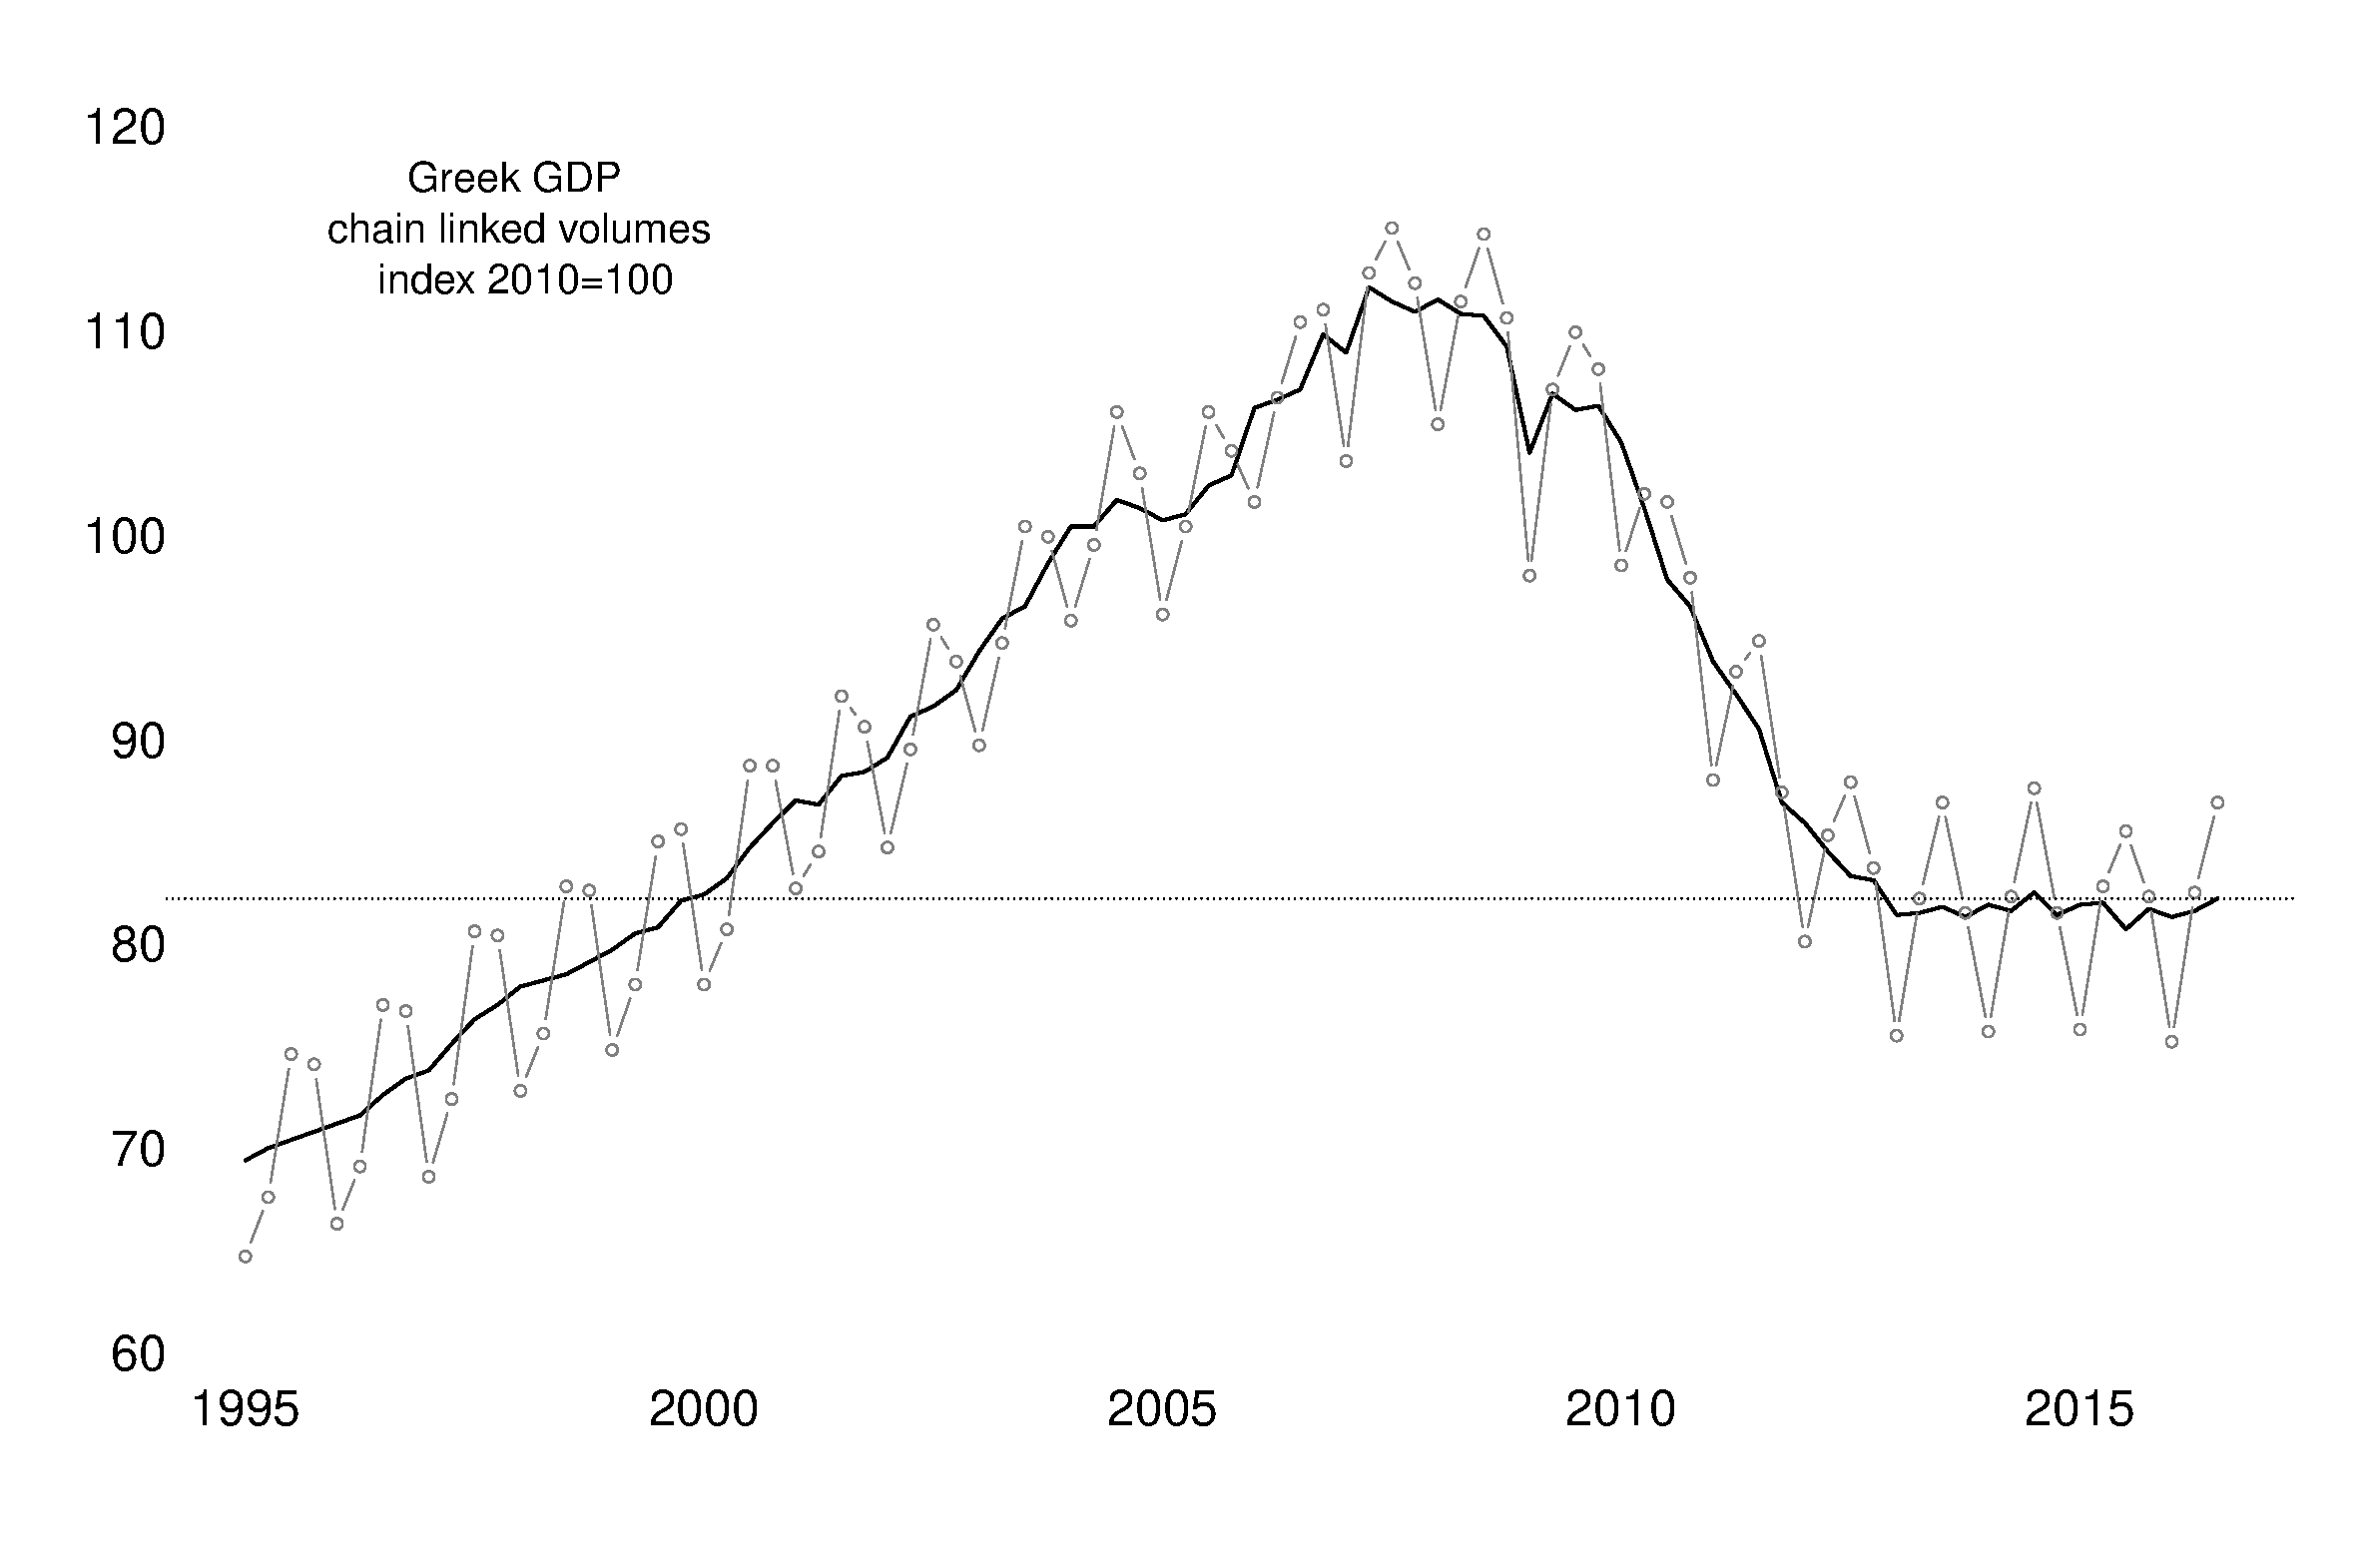
\includegraphics[scale=.3]{greece1.eps}
  \end{figure}
\end{frame}
%--------------------------------------

%--------------------------------------
\begin{frame}
  \begin{figure}
    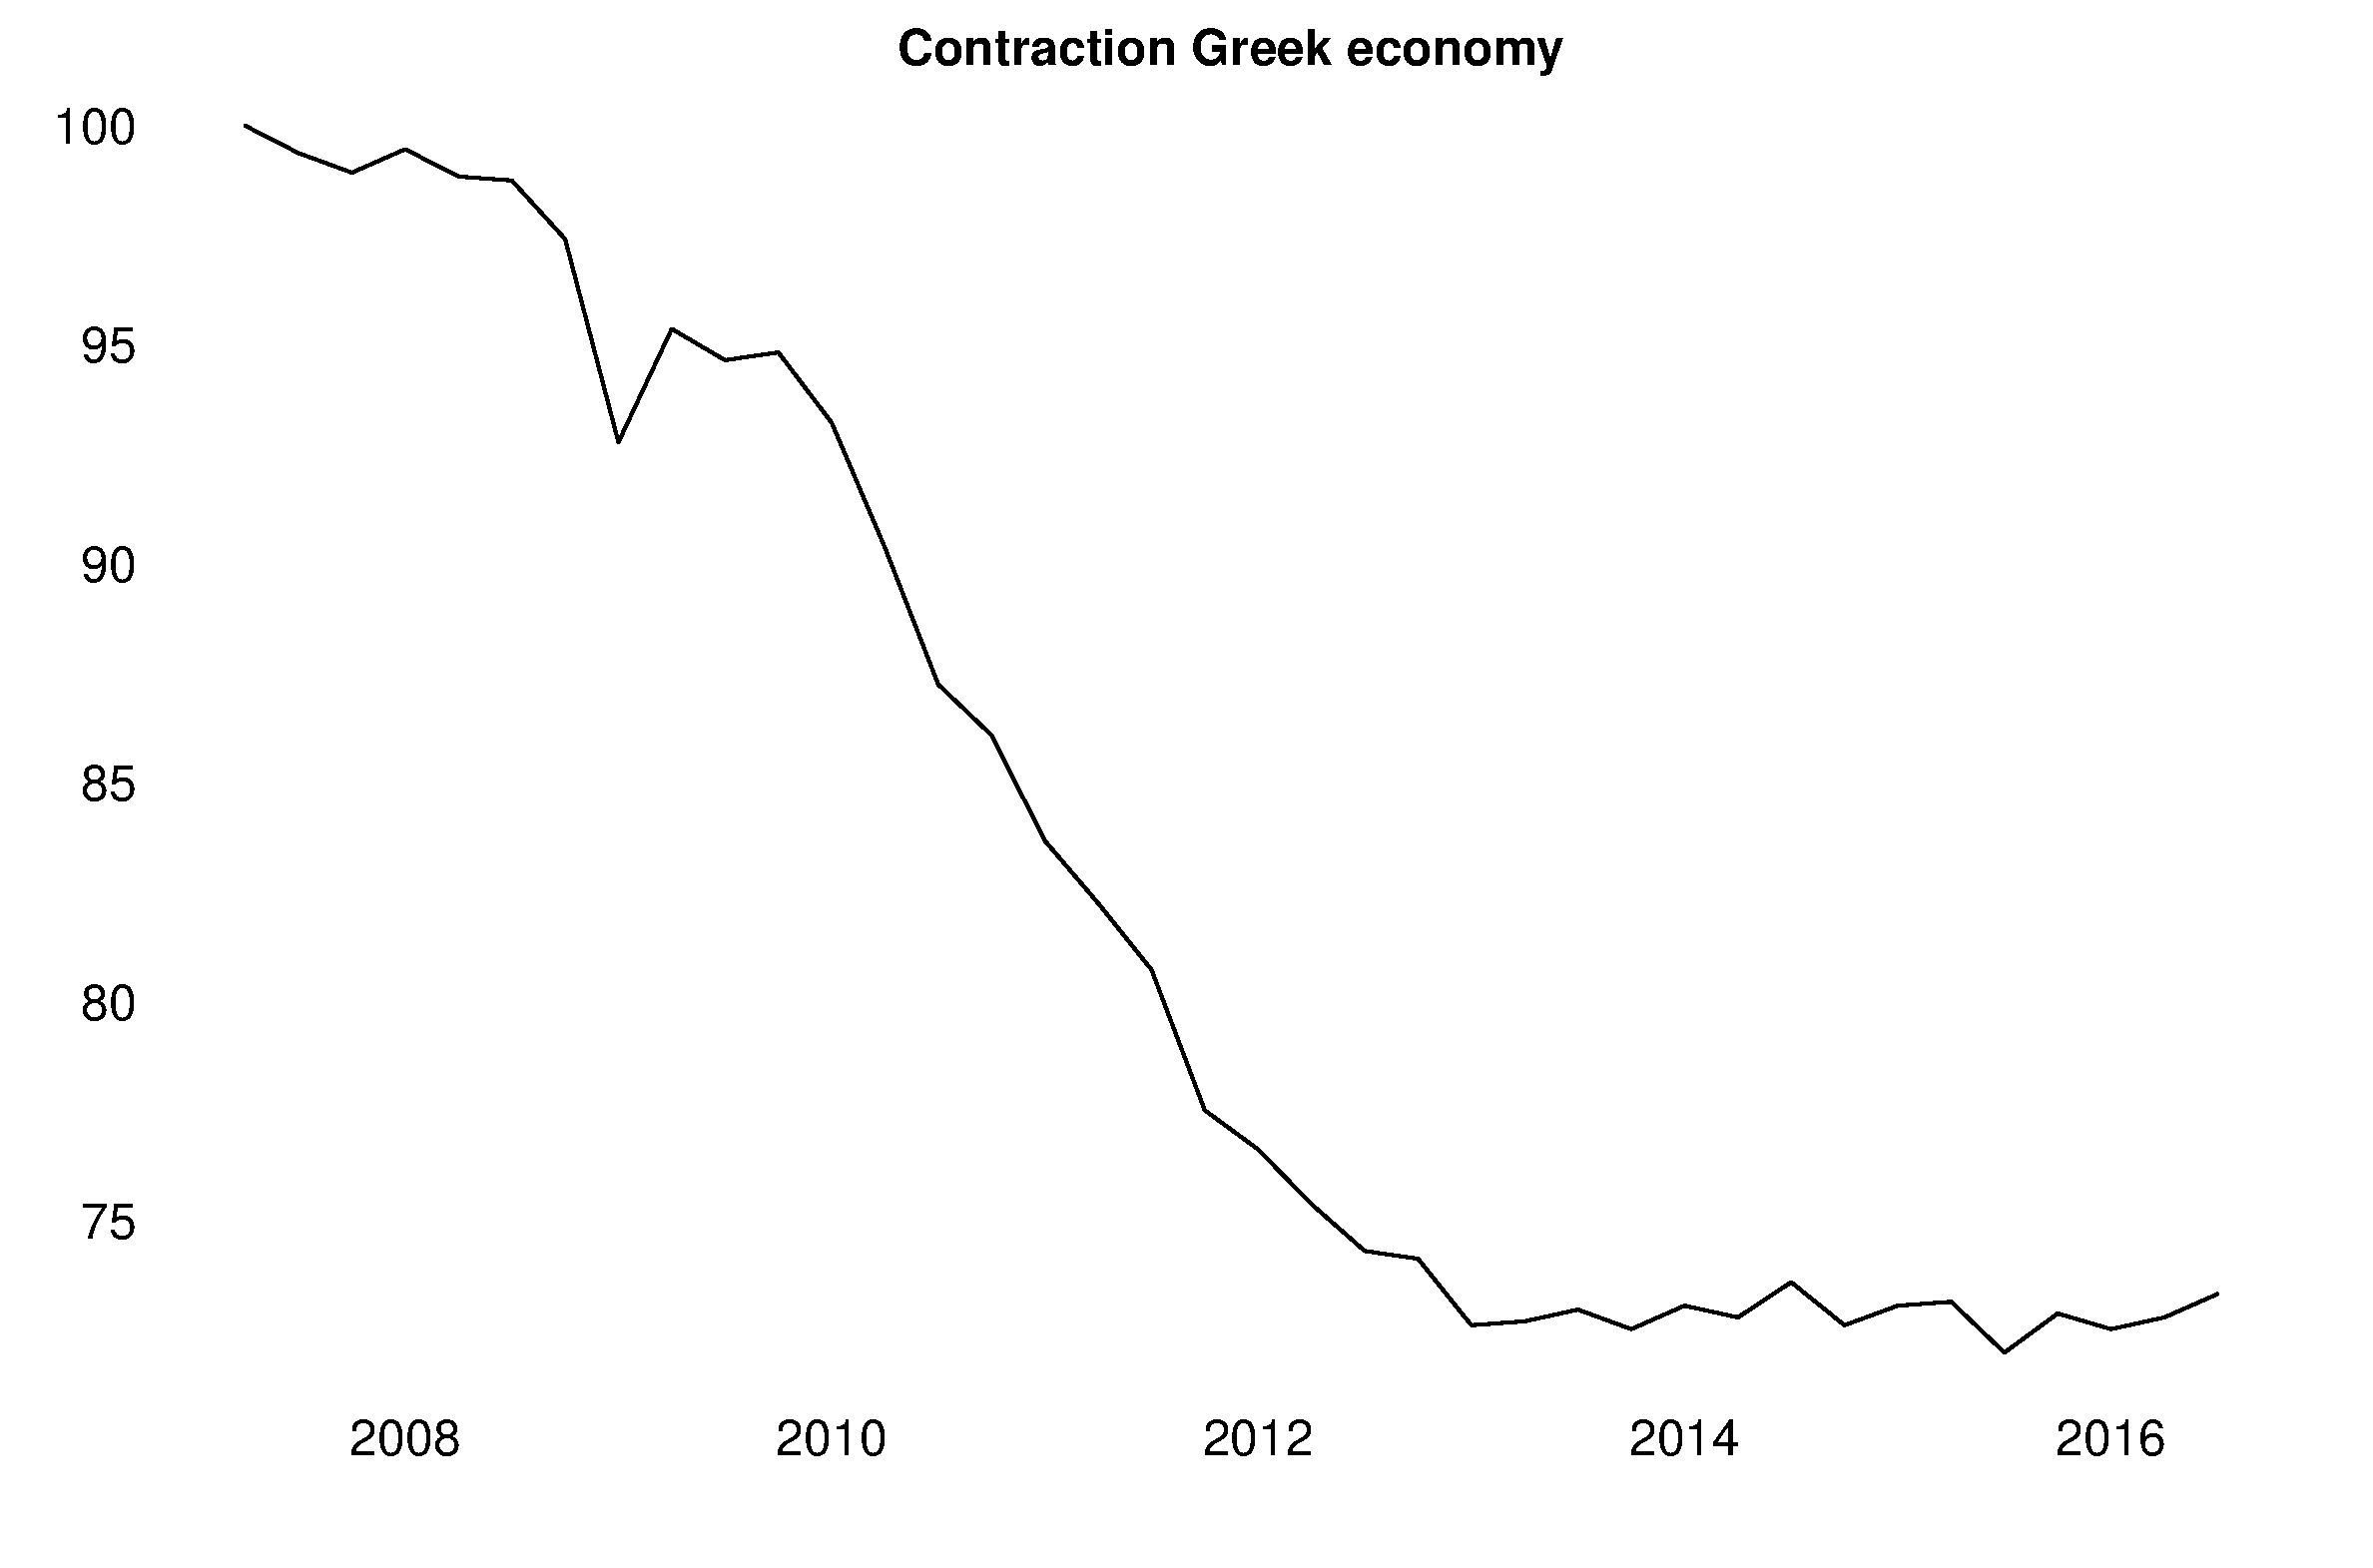
\includegraphics[scale=.3]{greece2.eps}
  \end{figure}
\end{frame}
%--------------------------------------

%--------------------------------------
\begin{frame}
  \textbf{Debt reduction schemes}
  \begin{enumerate}
    \item Unilateral debt forgiveness
    \item Third party buy-backs
    \item Debt restructuring (haircut)
    \item Debt swaps
    \item Default (nuclear option)
  \end{enumerate}  
\end{frame}
%--------------------------------------

%--------------------------------------
\begin{frame}
  \textbf{Greek debt reduction scheme}
  \begin{itemize}
    \item \textbf{21 Jan. 2010} Greek-German spread for 10-y debt reaches 300 basis points
    \begin{itemize}
      \item Default only option without outside help
    \end{itemize}
    \item \textbf{2 May 2010} Troika agree to 140B EUR bail-out package
    \begin{itemize}
      \item Guarantee Greek public debt: debt swap
    \end{itemize}
    \item \textbf{27 Oct. 2011} Major private bond holders agree on haircut
    \begin{itemize}
      \item 50\%, 83.5\% of Greek bond holders participate
    \end{itemize}
    \item \textbf{2012-2014} Arrangement becomes third party buy-back: ECB buys out large fraction and lowers interest rates
  	\item \textbf{Feb. 2014} Greek debt/GDP >170\%: Greece hopes for debt forgiveness from Troika
  	\item \textbf{2015} Greece defaults on IMF loan
  \end{itemize}
\end{frame}
%--------------------------------------

%--------------------------------------
\begin{frame}
  \textbf{Sovereign defaults}, how does that happen?\\
  Imagine the following for a country
  \begin{enumerate}
    \item 10\% chance of a default over the next year
    \item Default over 50\% of outstanding debt
  \end{enumerate}
 Country has to pay a 5\% premium on debt relative to safe assets.
 \begin{itemize}
   \item Extra premium will place an additional burden on the government
   \item Interest costs could rise above the funds that country can access to pay off the interest payments
   \item  Alternatively the country's GDP could expand in order to keep debt stable
 \end{itemize}
Market for government bonds might cease to operate as the country is deemed not credit-worthy, which means an increase in the risk of default going from unlikely to likely. 
\begin{itemize}
  \item It is important to note that the closing of a bond market is an rare and abrupt events. 
  \item Sovereign defaults are pretty rare as most developed economies are relatively stable. 
\end{itemize}
After a default a country needs to restructure it debt which often involves writing off part of it, in order to restore the debt level to a more sustainable level.
\end{frame}
%--------------------------------------

%--------------------------------------
\begin{frame}
  \textbf{Terms and conditions apply}
  \begin{itemize}
    \item Harsh austerity terms 
  \begin{itemize}
    \item Cuts in public spending such as investments 
    \item Tax increases    
  \end{itemize}
  \item Government overhaul
  \begin{itemize}
    \item Reducing size of the government apparatus
    \item Cutting back on pensions
    \item Importantly there were no cuts to defense spending in terms of percentage GDP    
  \end{itemize}
  \item Ending tax evasion by its citizens
  \item Making business in Greece easier  
  \end{itemize}
\end{frame}
%--------------------------------------

%--------------------------------------
\begin{frame}
  \begin{figure}
    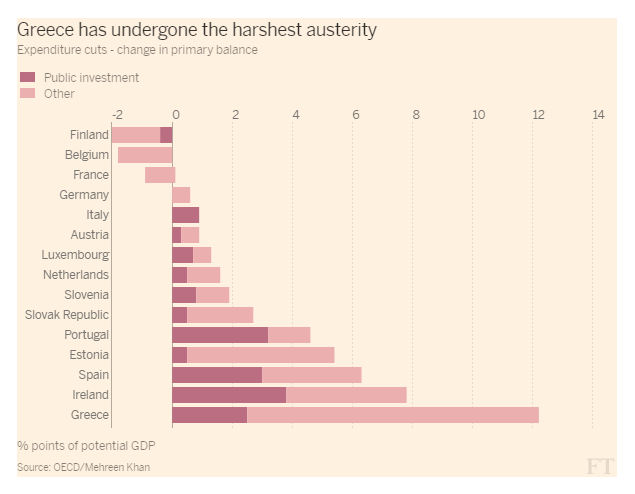
\includegraphics[scale=.3]{austerity.eps}
  \end{figure}
\end{frame}
%--------------------------------------

%--------------------------------------
\begin{frame}
  \begin{figure}
    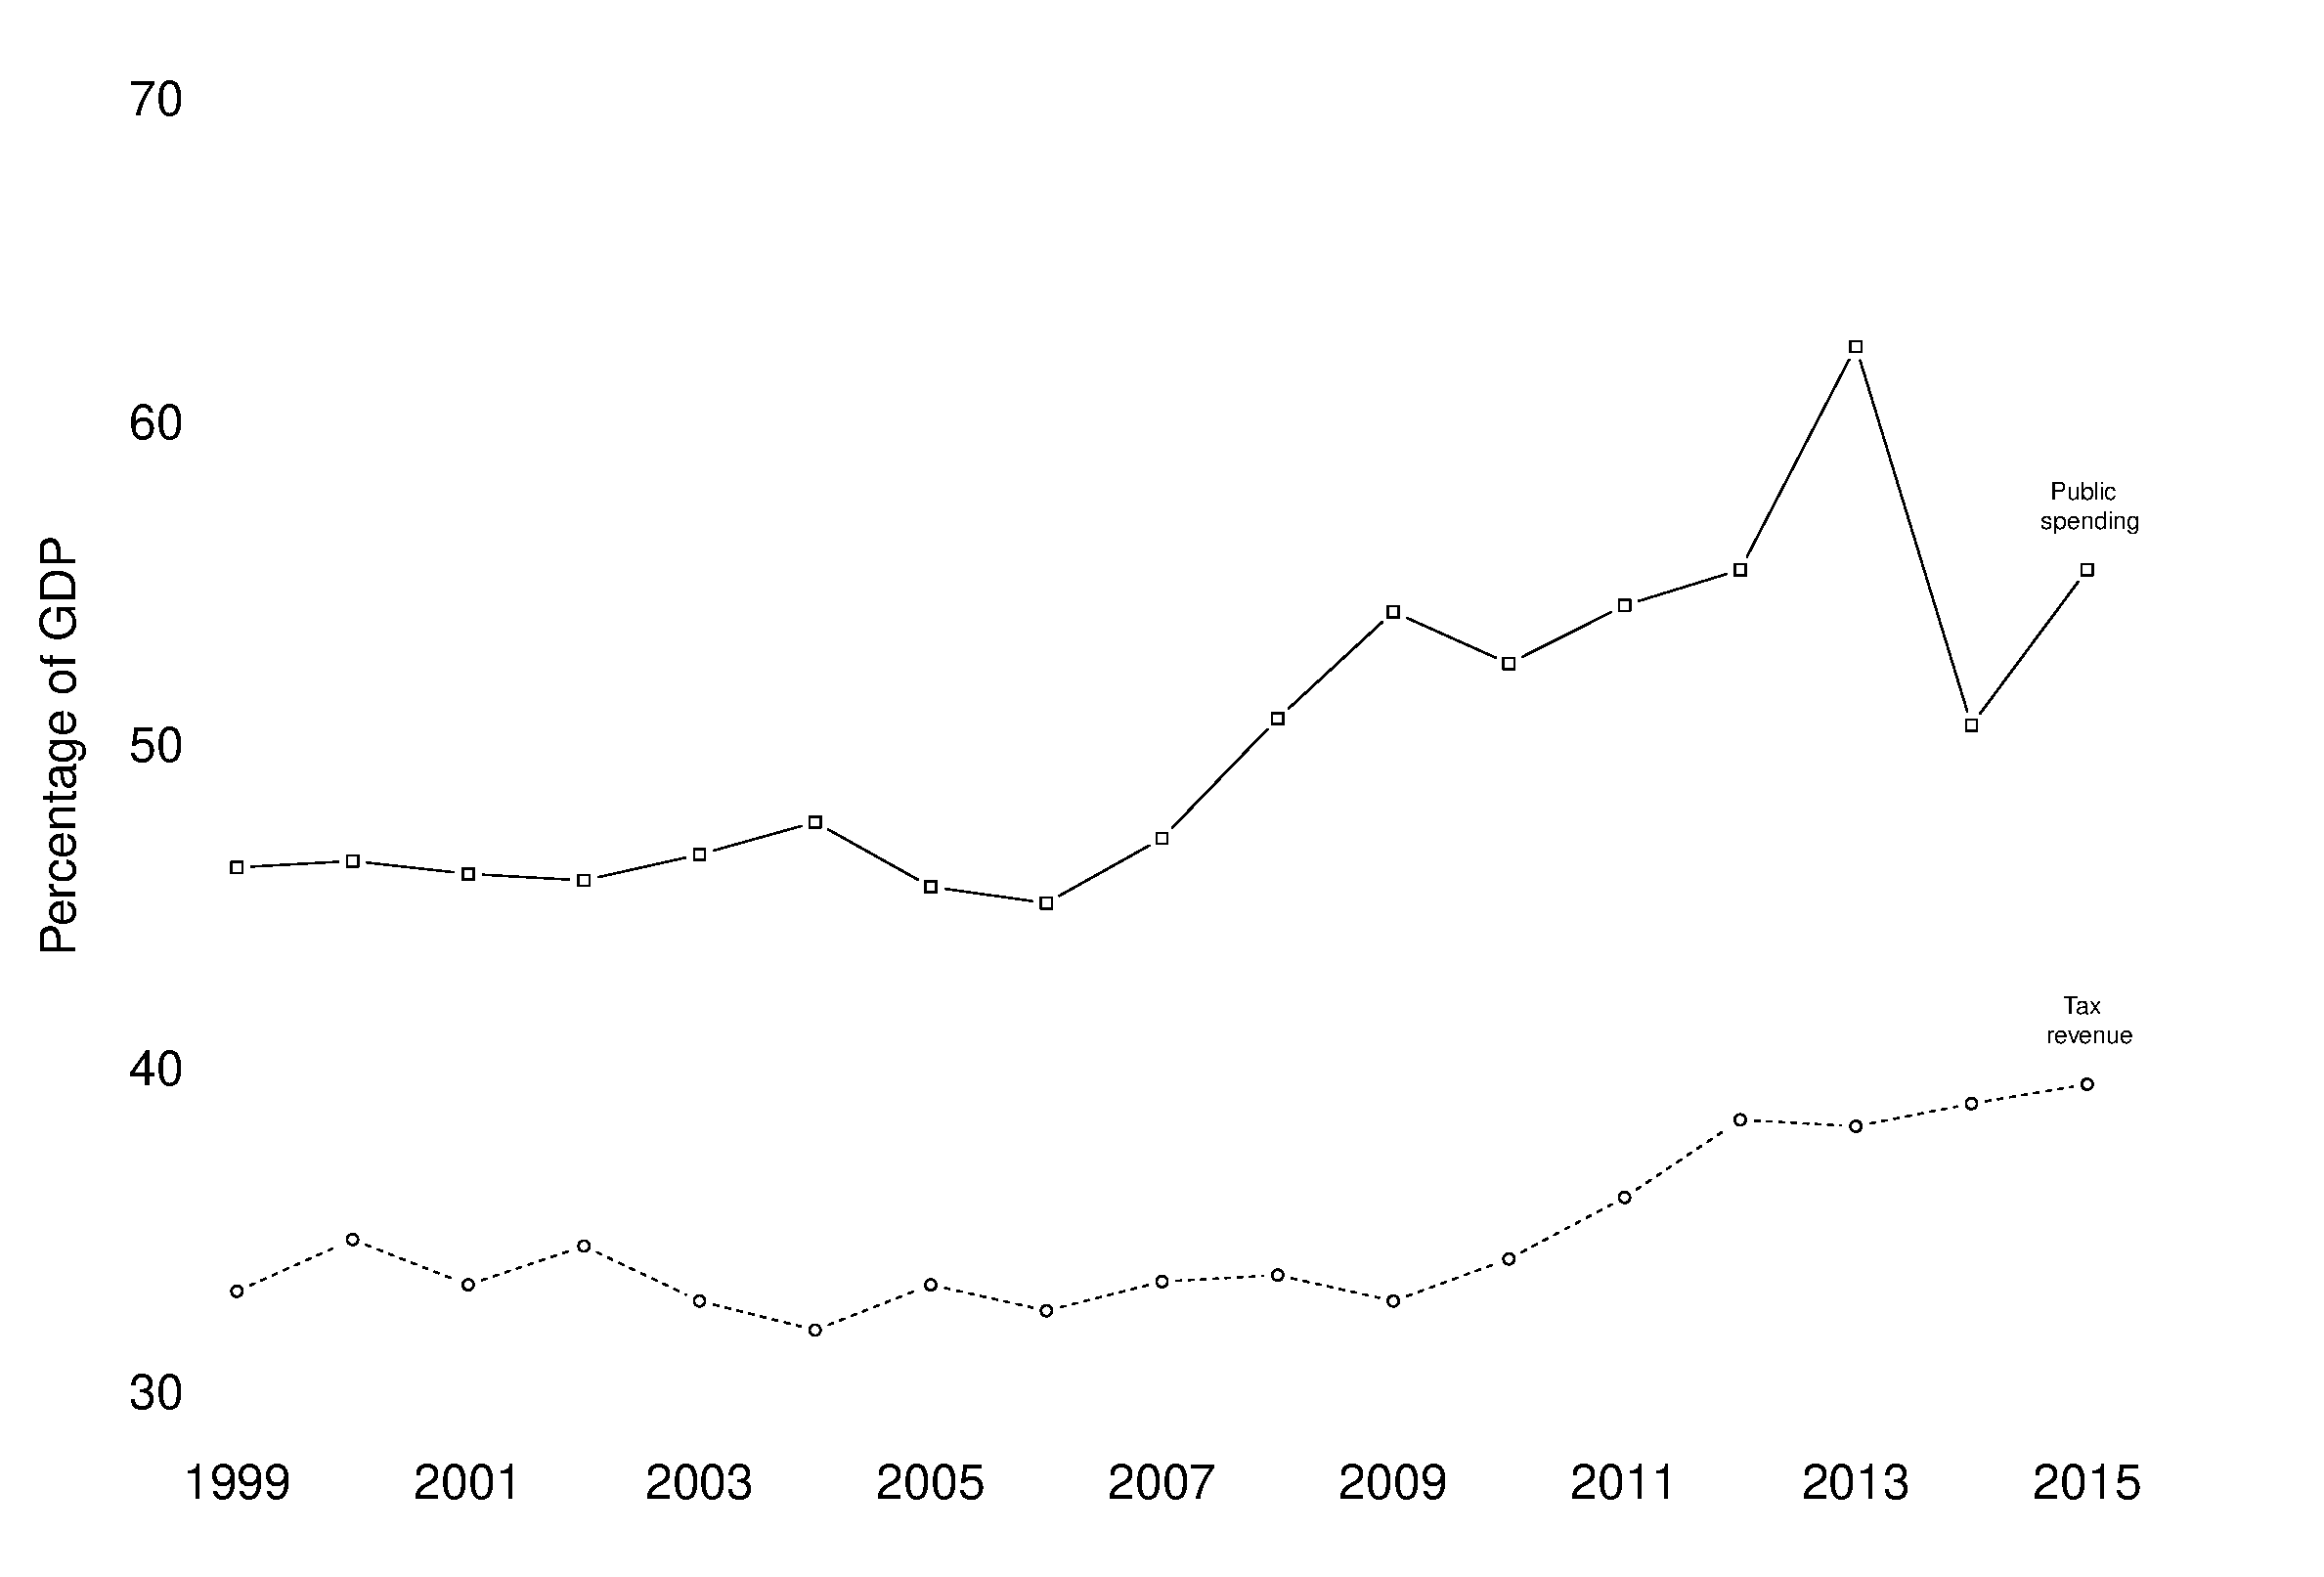
\includegraphics[scale=.3]{greece3.eps}
  \end{figure}
\end{frame}
%--------------------------------------

%--------------------------------------
\begin{frame}
  \begin{figure}
    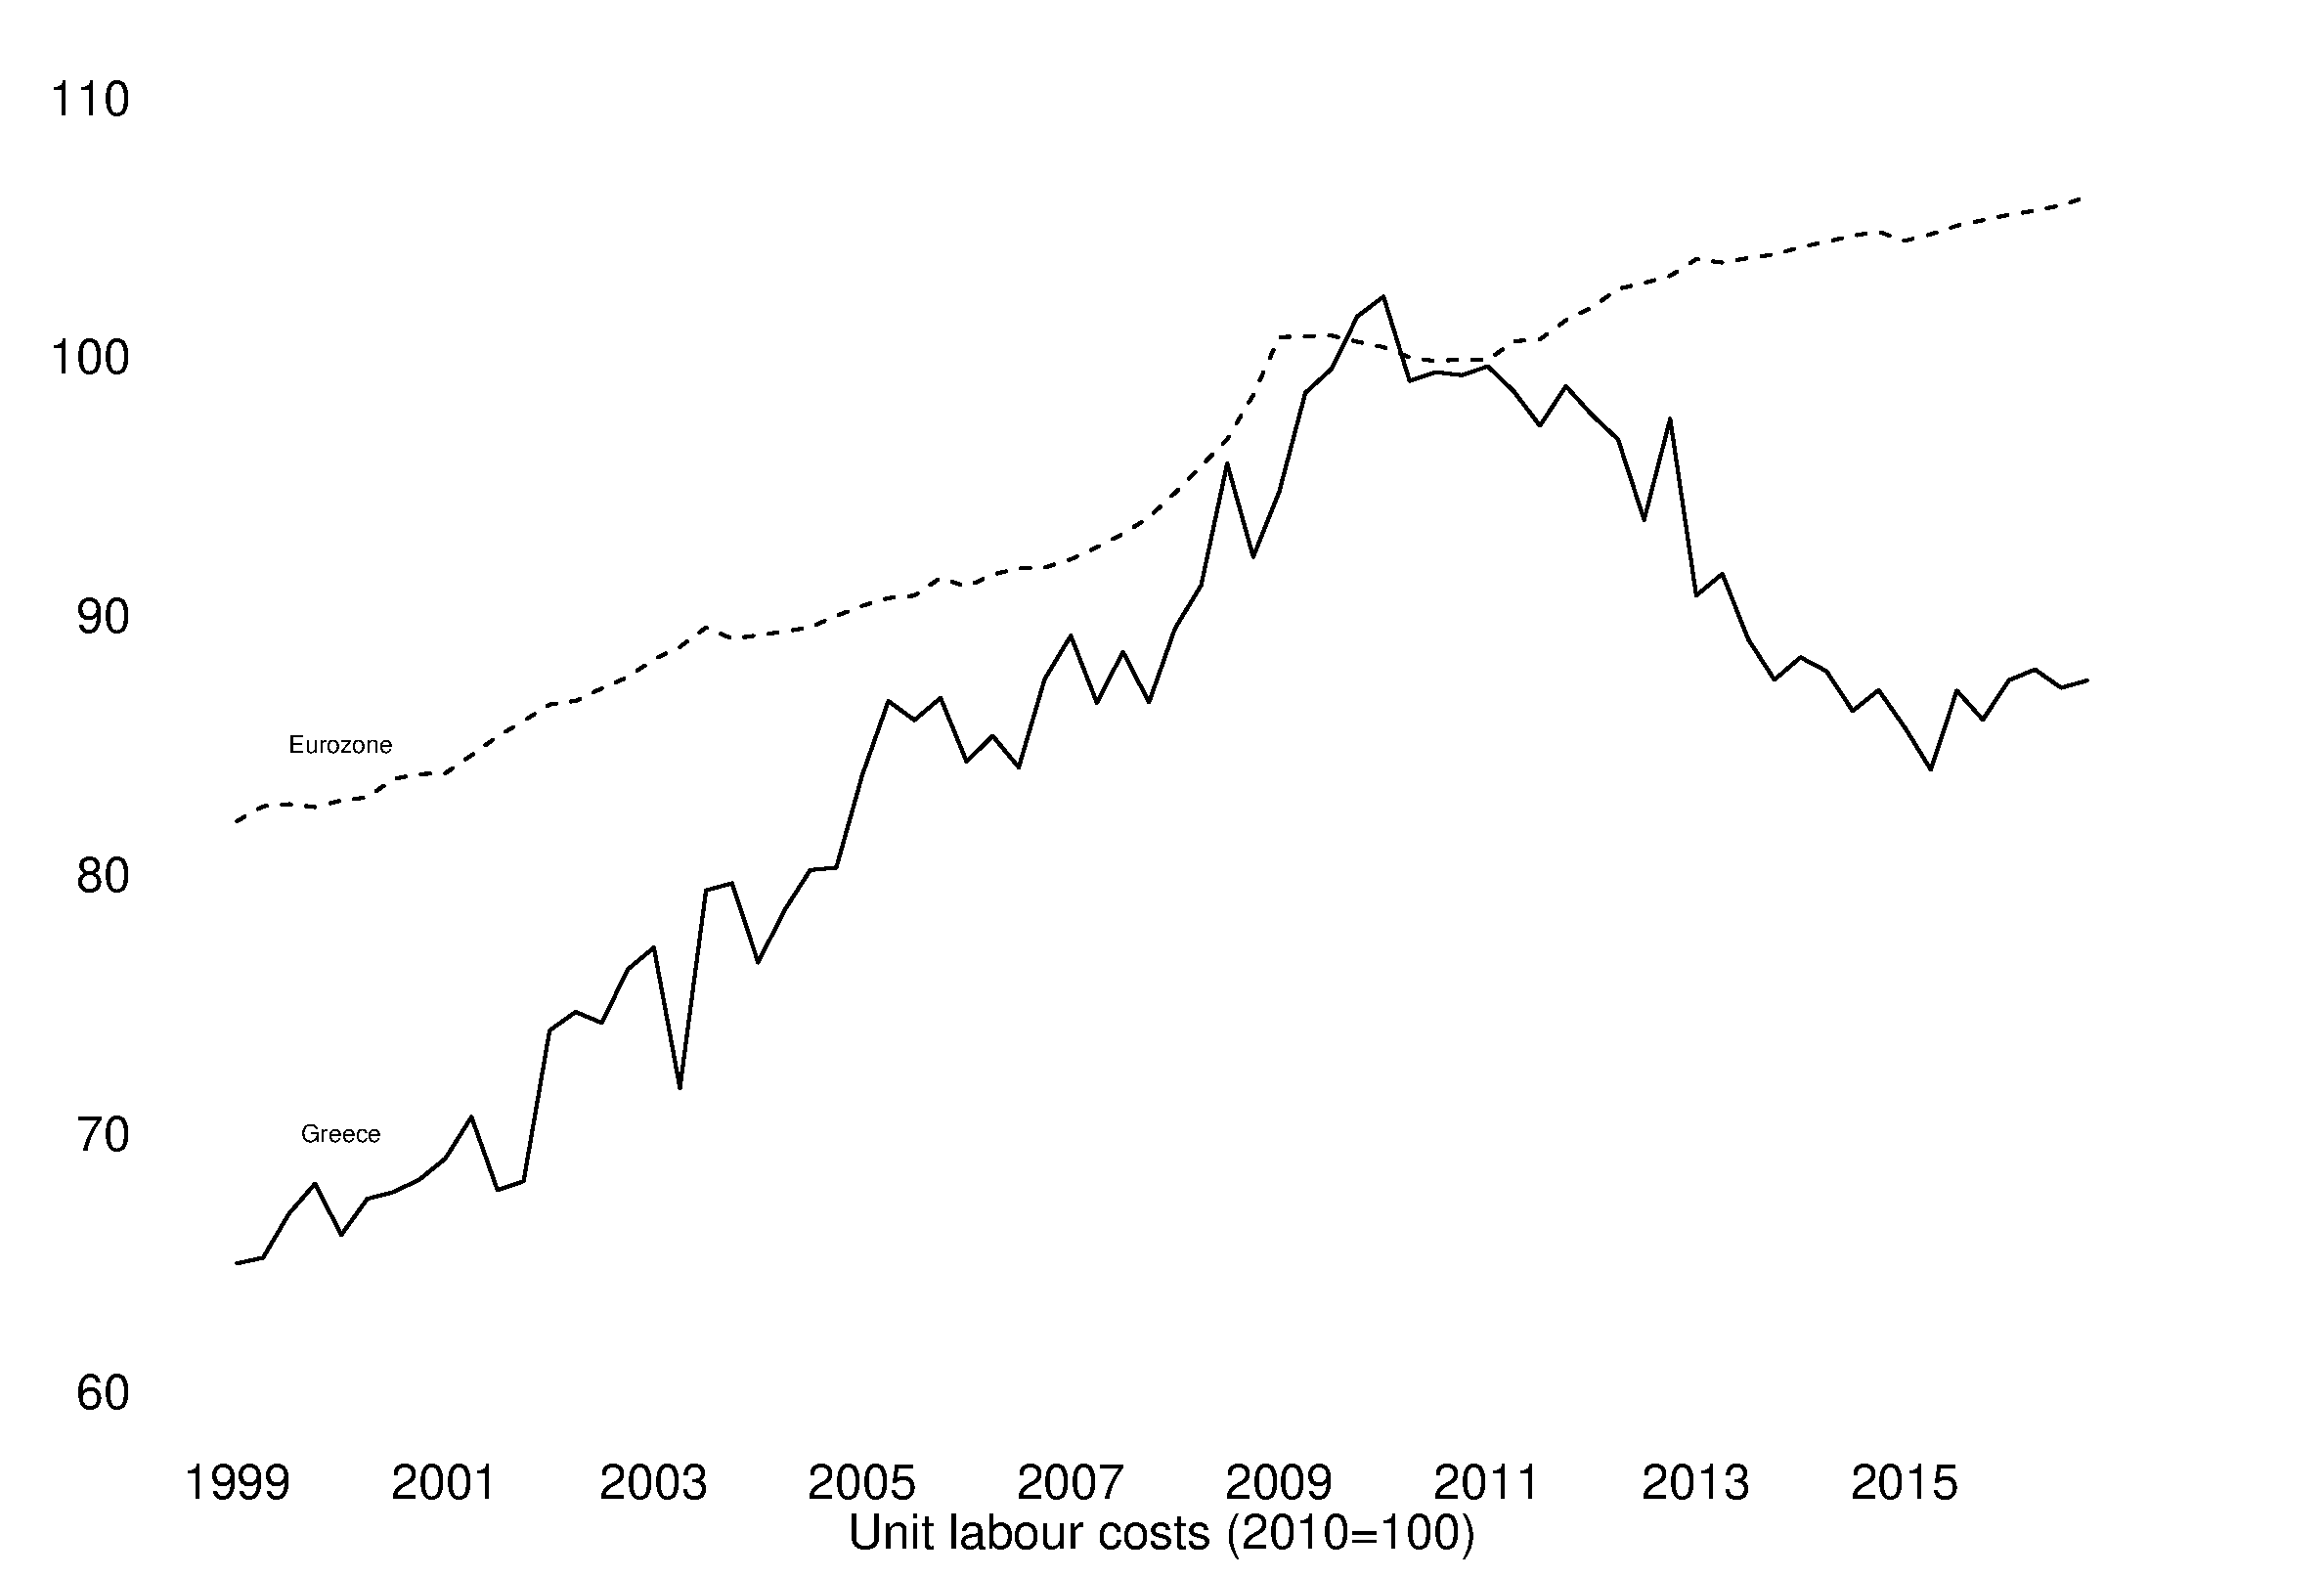
\includegraphics[scale=.3]{greece4.eps}
  \end{figure}
\end{frame}
%--------------------------------------

%--------------------------------------
\begin{frame}
  \begin{figure}
    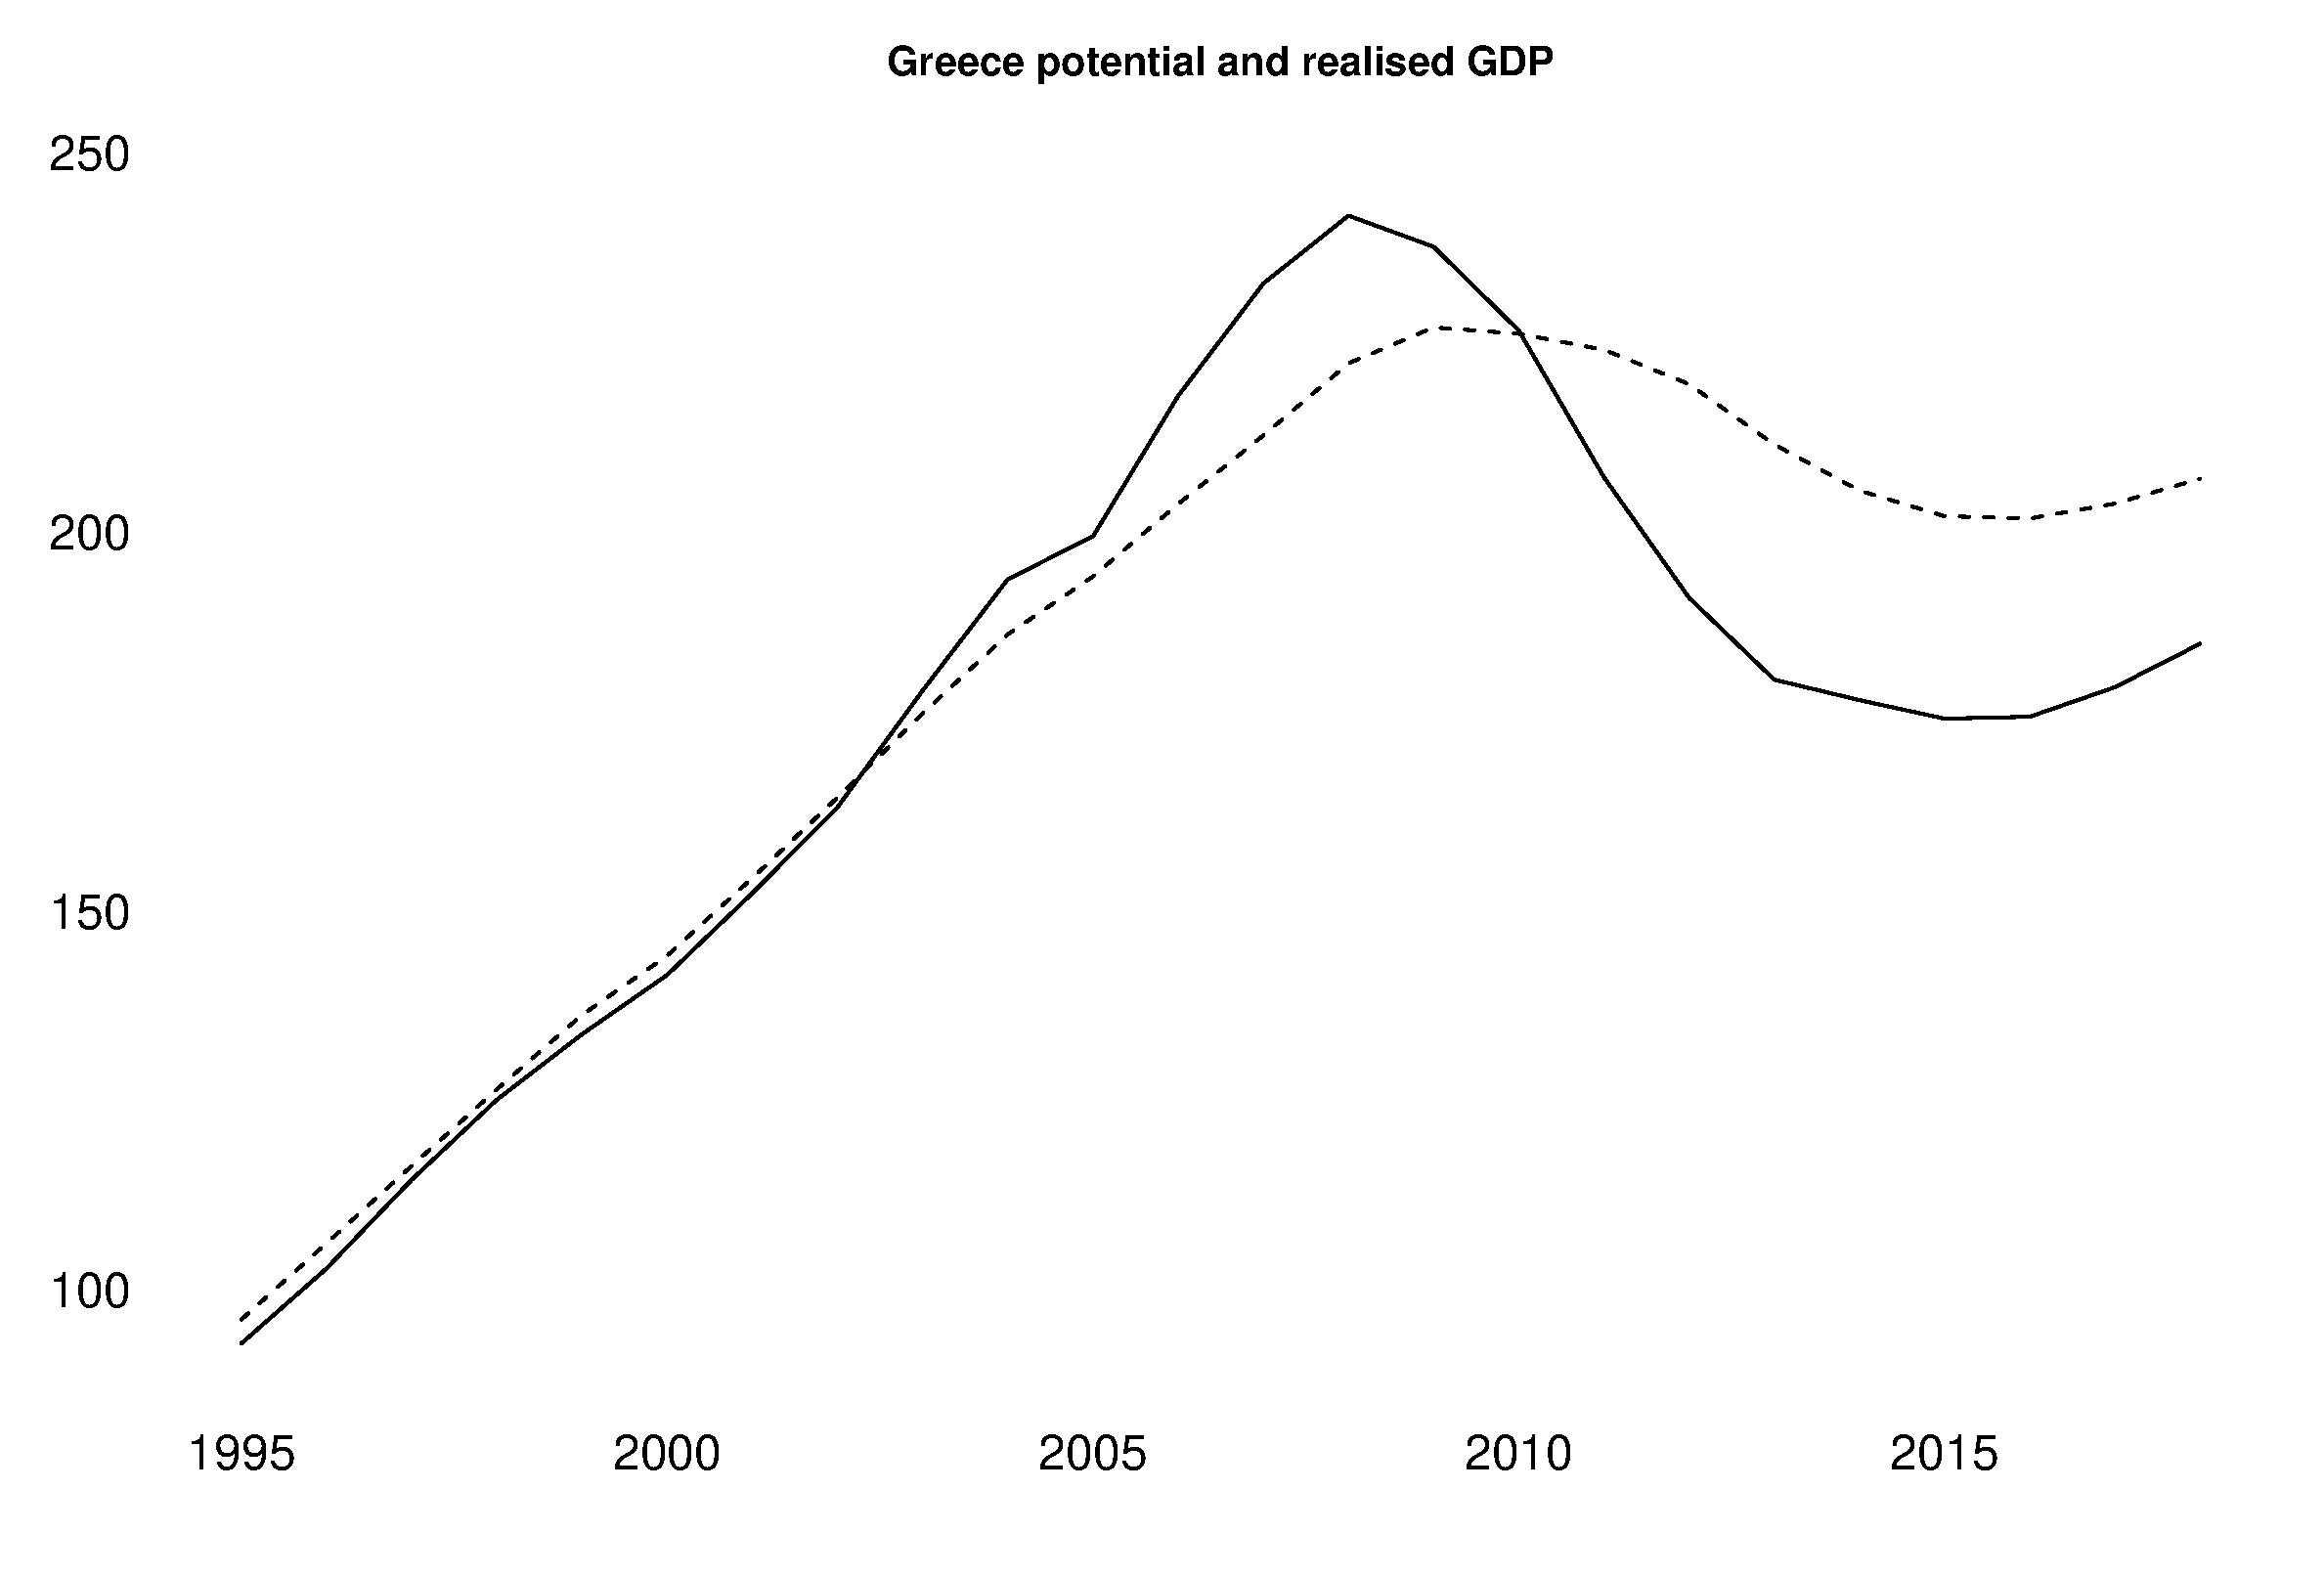
\includegraphics[scale=.3]{greece5.eps}
  \end{figure}
\end{frame}
%--------------------------------------


%--------------------------------------
\begin{frame}
  \textbf{ECB response} to eurocrisis\\
   Given its original mandate, the ECB's preferred course of action is to do nothing at all, and let governments sort out the mess.
   \begin{itemize}
      \item Recall that the ECB is independent, in order to limit government interference in its policy
    \end{itemize} 
    However, as the crisis progressed and got worse they had to come into action at some point. 
    \begin{itemize}
      \item A main fear was the risk of contagion from smaller, peripheral economies, such as Greece and Portugal, to larger central ones such as Italy and possibly France.
      \item Risk of contagion was a serious issue as for instance Italy owed France about 20\% of French GDP
    \end{itemize}
\end{frame}
%--------------------------------------

%--------------------------------------
\begin{frame}
  ECB took two measures
  \begin{enumerate}
    \item Standard
  \begin{itemize}
    \item Adjusting the key interest rates downwards
    \item Taken due to the macroeconomic circumstances and the risk for price stability
    \item Short-term interest rates are close to zero at the moment
  \end{itemize}
  \item Non-Standard
  \begin{itemize}
    \item Measures include fixed rate lending, providing longer maturity liquidity, expanding set of assets that can serve as collateral
    \item Taken because the banking system wasn't functioning properly
    \item ECB wanted to have a proper transmission of their monetary policy    
  \end{itemize}
  \end{enumerate}
\end{frame}
%--------------------------------------

%--------------------------------------
\begin{frame}
  ECB took a number of unconventional steps to show the commitment of the bank to guaranteeing the stability of the Eurozone
\begin{itemize}
  \item Long Term Refinancing Operations (LTRO)
  \begin{itemize}
    \item ECB committed itself to refinancing operations for multiple years, rather than couple of months which is common    
     \item ECB serves as lender of first resort to troubled banks, these banks could then help struggling governments by purchasing debt    
  \end{itemize}
  \item Securities Market Program (SMP)
  \begin{itemize}
    \item Purchasing government and private debt, from countries facing problems
    \item Similar to QE, main difference is that ECB keeps the books balanced; offsetting the purchases by offering the banks interest-bearing deposits
  \end{itemize}
  \item Outright Money Transactions (OMT)
  \begin{itemize}
    \item Under certain circumstances a state could request the ECB to buy bonds     
    \item OMTs haven't been used yet as none of the candidate countries met the criteria
  \end{itemize}
\end{itemize}
\end{frame}
%--------------------------------------

%--------------------------------------
\begin{frame}
  The process of economic and monetary integration in the EU is all about convergence of economic performance; raising living standards. 
For a time this process seemed to have paid off during the boom years in the first decade of the 21st century, but it unravelled quickly in the years after the crisis. 
Again focusing on a number of macroeconomic indicators we can illustrate how the crisis led to a divided Europe. 
\end{frame}
%--------------------------------------


%--------------------------------------
\begin{frame}

\end{frame}
%--------------------------------------

%--------------------------------------
\begin{frame}

\end{frame}
%--------------------------------------

%--------------------------------------
\begin{frame}

\end{frame}
%--------------------------------------

%--------------------------------------
\begin{frame}

\end{frame}
%--------------------------------------








%--------------------------------------
\end{document}

